\documentclass{article}
\usepackage[fontsize=13pt]{fontsize}
\usepackage[utf8]{inputenc}
\usepackage[sfdefault]{roboto}
\usepackage[T1]{fontenc}
\usepackage[ngerman]{babel}
\usepackage{amsmath,amsfonts,amssymb,amstext,esdiff}
\usepackage{geometry}
\usepackage{parskip}
\usepackage{svg}
\usepackage{float}
\usepackage{afterpage}
\usepackage{listings}
\usepackage{pdfpages}
\usepackage{hyperref}
\usepackage{cleveref}
\usepackage{multirow}
\usepackage{xltabular}
\usepackage{wrapfig}
\usepackage{fancyhdr}
\usepackage{caption}
\usepackage[framemethod=default]{mdframed} % Required for comment environment
\usepackage{tikz}
\usepackage[automake,toc,section=section]{glossaries}


\gdef\contentsname{Inhaltsverzeichnis}
\gdef\listfigurename{Abbildungsverzeichnis}
\gdef\listtablename{Tabellenverzeichnis}
%!TEX option = --shell-escape

\definecolor{dmGreen}{HTML}{009661}
\definecolor{htmlBlue}{HTML}{0060ff}

\definecolor{ocre}{RGB}{243,102,25}
\definecolor{codegreen}{rgb}{0,0.6,0}
\definecolor{codegray}{rgb}{0.5,0.5,0.5}
\definecolor{codepurple}{rgb}{0.58,0,0.82}
\definecolor{backcolour}{rgb}{0.95,0.95,0.92}
\lstdefinestyle{mystyle}{
commentstyle=\color{codegreen},
keywordstyle=\color{magenta},
numberstyle=\tiny\color{codegray},
stringstyle=\color{codepurple},
basicstyle=\ttfamily\footnotesize,
breakatwhitespace=false,
breaklines=true,
captionpos=b,
keepspaces=true,
numbers=left,
numbersep=5pt,
showspaces=false,
showstringspaces=false,
showtabs=false,
tabsize=2
}

\lstset{style=mystyle}
\geometry{
    a4paper,
    left=25mm,
    right=25mm,
    top=10mm,
    bottom=10mm,
    includeheadfoot,
    heightrounded
}

\newcommand{\argmin}[1]{\underset{#1}{\operatorname{argmin}}}
\newcommand{\para}[1]{\vspace{-5mm}\subsubsection*{#1}\vspace{-4mm}}

\renewcommand{\baselinestretch}{1.2}

% \renewcommand*{\arraystretch}{1.4}
\captionsetup[figure]{labelfont={bf},name={Figure}} % Caption title for figures/images
\captionsetup[table]{labelfont={bf},name={Table}}
\setlength{\belowcaptionskip}{-6pt} % reduce padding/mardin below figure and table captions

\hypersetup{
    colorlinks=true,
    anchorcolor=black,
    citecolor=htmlBlue, % citations
    linkcolor=htmlBlue, % in-document links
    filecolor=black,
    urlcolor=htmlBlue, % \href{URL}{text} usages
    pdftitle={D6_Lastenheft_Pong},
    pdfauthor={Leon Wiesen}
}

\setcounter{secnumdepth}{5}
\setcounter{tocdepth}{5}

\pagestyle{fancy}
\fancyhf{}
\lhead{\rightmark}
\rhead{Lastenheft "Pong"}
\cfoot{\thepage}


\makeglossaries
\newglossaryentry{muss}{ name={muss}, description={
    Diese Funktion ist verbindlich.
}}
\newglossaryentry{sollte}{ name={sollte}, description={
    Diese Funktion ist optional und wird implentiert wenn die notwendigen Ressourcen zur Verfügung stehen.
}}
\newglossaryentry{balken}{ name=Balken, description={
    Das einzige Spielelement, welches der Spieler aktiv kontrollieren kann. Positioniert am unteren Bildschirmrand, prallt der
    Ball von diesem horizontalen Balken ab und kann über das Spielfeld bewegt werden.
}}
\newglossaryentry{ball}{ name=Ball, description={
    Das zentrale Spielelement, welches vom Balken und von allen Rändern des Spielfelds abprallt und durch die physikalische
    Interaktion mit dem Balken indirekt vom Spieler gesteuert wird.
}}
\newglossaryentry{beta}{name={Beta-Version},description={
    Eine vorläufige und funktionstüchtige Testversion des Spiels, die der Erhaltung von Feedback dient und diesem dynamisch angepasst wird.
}}
\newglossaryentry{block}{ name=Block, description={
    Ein Spielobjekt, welches im \gls{invasionMode} vom \gls{ball} zerstört werden muss.
}}
\newglossaryentry{classicMode}{ name=Classic-Mode, description={
    Der klassische Pong-Spielmodus, bei dem nur ein \gls{ball} und ein \gls{balken} auf dem \gls{spielfeld} existiert.
}}
\newglossaryentry{coin}{ name=Coin, description={
    Die Währung des Spiels.
}}
\newglossaryentry{invasionMode}{ name=Invasion-Mode, description={
    Ein erweiterter Spielmodus, bei dem der \gls{ball} zusätzlich \gls{block}-Objekte zerstört.
}}
\newglossaryentry{ladezeiten}{ name=Ladezeiten, description={
    Die Wartezeit beim initialen Laden der App (Starten aus dem Betriebssystem) und Wechsel zwischen Menüs.
}}
\newglossaryentry{leben}{ name=Leben, description={
    Eine abstrakte Währung, die der Beendigung eines Spieldurchlaufs dient. Besitzt der \gls{spieler} keine Leben mehr, endet das Spiel.
}}
\newglossaryentry{niceToHave}{ name=Nice-To-Have, description={
    Optionale Anforderungen, die nicht rechtlich bindend und deren Implementierung völlig dem Entwicklerteam überlassen sind.
}}
\newglossaryentry{powerup}{ name=Power-Up, description={
    Ein temporärer Effekt, der z.B. Spielelemente wie den Ball oder den Balken betrifft und deren Verhalten ändert.
}}
\newglossaryentry{release}{name={Release-Version},description={
    Die finale und ausgelieferte Version des Spiels.
}}
\newglossaryentry{tail}{ name=Schweif, description={
    Kosmetikeffekt hinter dem Ball, welcher die Bahnkurve anzeigt. Gleicht dem Schweif einer Sternschnuppe.
}}
\newglossaryentry{point}{ name=Score-Point, description={
    Ein Wert, der dem \gls{spieler} als Metrik für seine Fähigkeiten dient. Im Verlauf des Spiels sammelt der \gls{spieler} zwangsläufig mehr.
}}
\newglossaryentry{skin}{ name=Skin, description={
    Kosmetikeffekte wie verschiedene Sprites/Texturen für Ball, Balken und Spielhintergrund.
    Diese können im Shop gegen Coins eingetauscht werden.
}}
\newglossaryentry{spieler}{ name=Spieler, description={
    Jede Person, die die Anwendung nutzt. \textit{Synonyme: Benutzer, Anwender}.
}}
\newglossaryentry{spielfeld}{ name=Spielfeld, description={
    Umfasst den Bereich, in dem das Spiel stattfindet. Vertikale Abgrenzungen sind der linke und rechte Bildschirmrand.
    Der obere Bildschirmrand bildet die obere Abgrenzung, die untere Abgrenzung erfolgt auf der Höhe, auf der sich der
    \gls{balken} befindet.
}}
\newglossaryentry{Top10}{ name=Top10, description={
    Die zehn besten Scores, die lokal auf einem Gerät (seit Installation) erreicht wurden.
}}
\newglossaryentry{achievements}{ name=Achivement, description={
    Errungenschaft, die der \gls{spieler} im Laufe des Spiels freischalten kann, welche weder funktionelle noch kosmetische Auswirkungen auf das Spielgeschehen haben.
}}



\begin{document}
\gdef\contentsname{Inhaltsverzeichnis}
\gdef\listfigurename{Abbildungsverzeichnis}
\gdef\listtablename{Tabellenverzeichnis}
    \pagenumbering{gobble}
    \selectlanguage{english}

    
\begin{titlepage} % Suppresses displaying the page number on the title page and the subsequent page counts as page 1
	\newcommand{\HRule}{\rule{\linewidth}{0.5mm}} % Defines a new command for horizontal lines, change thickness here
	
	\center % Centre everything on the page
	
	%------------------------------------------------
	%	Headings
	%------------------------------------------------
	
	\textsc{\LARGE Software Engineering WS22/23}\\[1.5cm] % Main heading such as the name of your university/college
	
	\textsc{\Large ISLCM Gruppe 8}\\[0.5cm] % Major heading such as course name
	
	\textsc{\large SWE Praktikumsgruppe D6}\\[0.5cm] % Minor heading such as course title
	
	%------------------------------------------------
	%	Title
	%------------------------------------------------
	
	\HRule\\[0.4cm]
	{\huge\bfseries Lastenheft: Mobile App "Pong"}\\[0cm] % Title of your document
	\HRule\\[0.4cm]
	
	%------------------------------------------------
	%	Author(s)
	%------------------------------------------------
	
    \begin{xltabular}{\linewidth}{l X r}
        \textbf{Projektmanagement} & & \textbf{Qualitätssicherung} \\
        Marc-André Hein         & & Dorian Ailin Hövelmann                  \\
        Felix Horn              & & Tobias Bogner               \\
        & & \\
        \textbf{Technologie}    & & \textbf{Vertrieb}           \\
        Markus Helm             & & Hristomir Dimov             \\
        Daniel-Michel Richter   & & Leon Wiesen                 \\
    \end{xltabular}
    \label{tab:table_of_members}
    
    
	% If you don't want a supervisor, uncomment the two lines below and comment the code above
	%{\large\textit{Author}}\\
	%John \textsc{Smith} % Your name
	
	%------------------------------------------------
	%	Date
	%------------------------------------------------
	
	\vfill\vfill\vfill % Position the date 3/4 down the remaining page
	
	\textbf{Version 1.0} \\
	\textit{06.11.2022} \\
	\vspace*{0.4cm}
	Vorgelegt von: \\
	Leon Wiesen
	%------------------------------------------------
	%	Logo
	%------------------------------------------------
	
	%\vfill\vfill
	%\includegraphics[width=0.2\textwidth]{placeholder.jpg}\\[1cm] % Include a department/university logo - this will require the graphicx package
	 
	%----------------------------------------------------------------------------------------
	
	\vfill % Push the date up 1/4 of the remaining page
	
\end{titlepage}


    \gdef\contentsname{Inhaltsverzeichnis}
    \tableofcontents
    \clearpage

    \section*{Changelog}\label{sec:changelog}
    \addcontentsline{toc}{section}{\protect\numberline{}Changelog}
    Die folgenden Änderungen wurden im Laufe der Entwicklung des Lastenhefts vollzogen. Diese erfolgten aus den Gesprächen und dem Schriftverkehr zwischen Kunden (siehe \hyperref[sec:auftraggeber]{Auftraggeber}) und dem Vertrieb (Hristomir Dimov \& Leon Wiesen).

\begin{xltabular}{\textwidth}{|c|X|}
    \hline
    \textbf{Version}   & \textbf{Änderungen}     \\
    \hline

    v0.1    &  \begin{itemize}
        \item Kap. \ref{sec:auftraggeber}: Hinzugefügt
        \item Kap. \ref{sec:zeitbudget}: Hinzugefügt
        \item Kap. \ref{sec:bestimmung}: Hinzugefügt
        \item Kap. \ref{sec:einsatz}: Hinzugefügt
        \item Kap. \ref{sec:funktionen}: Neue MockUps
        \item Kap. \ref{sec:produktdaten}: Hinzugefügt
        \item Kap. \ref{sec:performance}: Hinzugefügt
        \item Kap. \ref{sec:quality}: Hinzugefügt
        \item Kap. \ref{sec:requirements}: Requirements erweitert
    \end{itemize}
    \\ \hline

    v1.0   & \begin{itemize}
        \item Allgemeine Rechtscheib- \& Grammatikfehler korregiert
        \item Glossar: Neue Begriffe Hinzugefügt
        \item Deckblatt: Gruppenname vervollständigt
        \item Kap. \ref{sec:auftraggeber}: Spezifischer formuliert
        \item Kap. \ref{sec:zeitbudget}: Glossar-Verlinkungen
        \item Kap. \ref{sec:einsatz}: Use-Case Diagramm hinzugefügt
        \item Kap. \ref{sec:funktionen}: Neue Diagramme
        \item Kap. \ref{sec:funktionen}: Genauere Beschreibungen
        \item Kap. \ref{sec:funktionen}: Glossar-Verlinkungen
        \item Kap. \ref{sec:performance}: Minimierung auf das Nötigste
        \item Kap. \ref{sec:abnahme}: Hinzugefügt
    \end{itemize}
    \\ \hline

\end{xltabular}
    \clearpage

    \pagenumbering{arabic}\setcounter{page}{1}

    \section{Auftraggeber}\label{sec:auftraggeber}
        Auftraggeber des Mobile Games "PONG" ist Gruppe 8 von Master-Studierenden (Kunden)
der FH Aachen - Fachbereich Elektrotechnik und Informationstechnik an der Eupener Straße 70 in D-52066 Aachen. Die Kunden belegen an der Hochschule das Modul "Information System Lifecycle Management". \\
Mit der in Auftrag gegebenen App möchte der Kunde einen Zeitvertreib/ein Gelegenheitsspiel für die breite Masse erhalten. Das nostalgische Gefühl des Klassikers soll auf dem großen Mobile-Markt erneut zum Leben erweckt und kostenlos zur Verfügung gestellt werden.
    \clearpage

    \section{Zeit- und Budgetrahmen}\label{sec:zeitbudget}
        
Das Mobile Game "PONG" wird im Wintersemester 2022/2023 im Rahmen der Lehrveranstaltung
"Software Engineering“ in dem Studiengang „Informatik” des Fachbereiches 5 (Elektrotechnik und
Informationstechnik) an der Fachhochschule Aachen entwickelt.
Der Fachbereich befindet sich in der Eupener Straße 70 in D-52066 Aachen.

Die finale Version dieses Dokumentes muss bis zum \textbf{11.11.2022} fertiggestellt und
von beiden Seiten unterzeichnet werden.

Bis zum \textbf{21.12.2022} muss eine \gls{beta} erstellt werden, die dem Kunden
vorgelegt werden kann. 
Die erste \gls{release} der Applikation muss bis Ende
des Wintersemesters 2022/23, zum \textbf{12.01.2023}, fertiggestellt und abgenommen werden.

Zur Fertigstellung des Projekts haben wir als Auftragnehmer ein Zeitbudget von 600 Stunden. 


\begin{figure}[h!]
    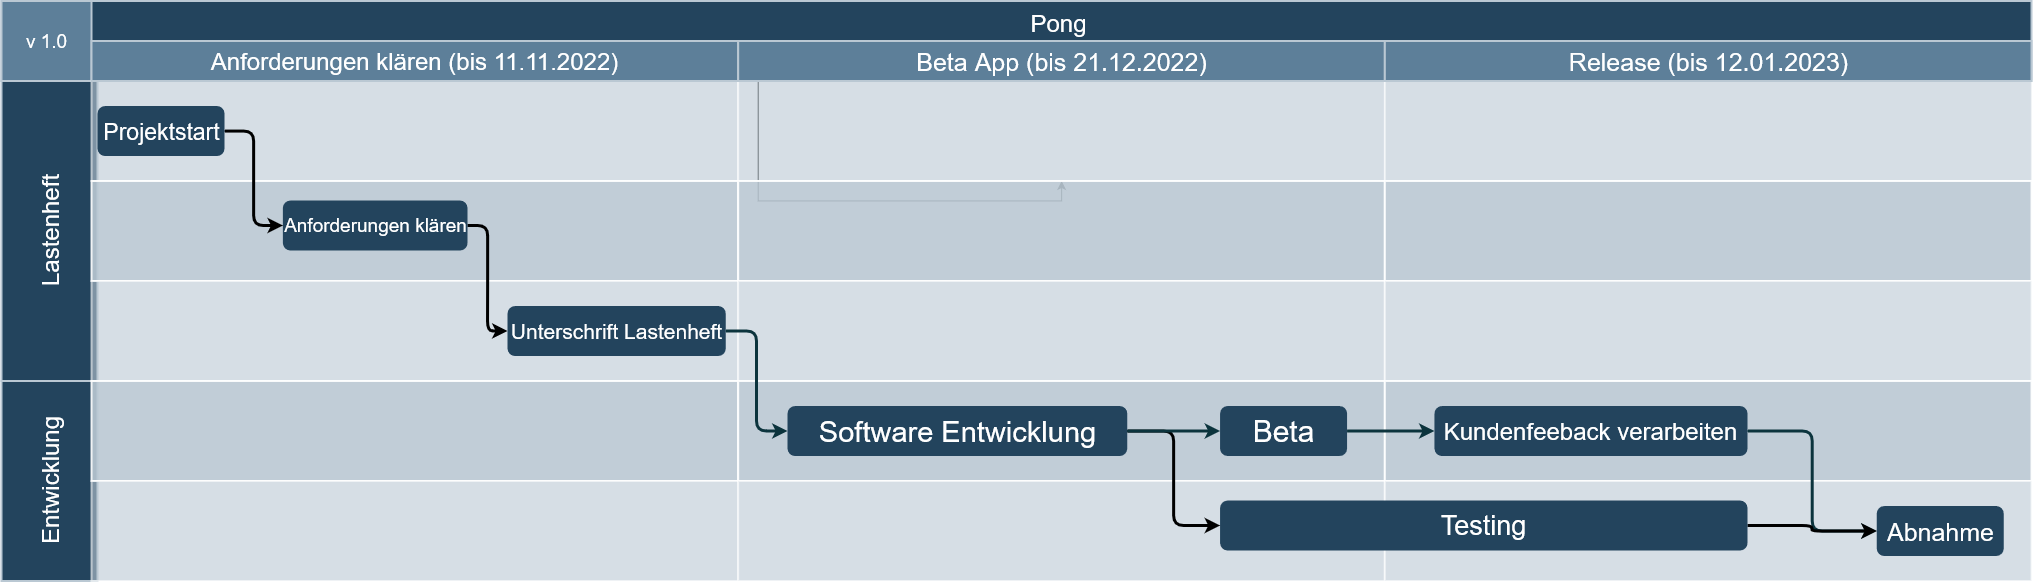
\includegraphics[width=\textwidth]{pics/ZeitlicherAblauf.png}
\end{figure}


    \clearpage

    \section{Zielbestimmung}\label{sec:bestimmung}
        \subsection{Zweck}
            Der Benutzer verwendet das Spiel „Pong“ als Gelegenheitsspiel, das z.B. in Pausen die Langeweile vertreibt. 
Des weiteren kann der Benutzer das Spiel verwenden um sich mit anderen durch Top-Scores zu messen oder um der Realität zu entfliehen und Spaß zu haben. 
Der gesellschaftliche Effekt des Austauschs von Highscores und bereits freischaltbare Items ist ebenfalls ein zentraler Punkt.
\\
Außerdem ist ein Zweck der Benutzung die stetige Verbesserung im Spiel.
"Pong" ist allerdings kostenlos erhältlich und kann von Menschen aus allen Lebensbereichen genossen werden.
        \subsection{Nutzen}
            Das Spiel „Pong“ ermöglicht es dem Spieler sich im Spiel zu verbessern, sich mit anderen zu konkurrieren und bei Gelegenheit der Realität entfliehen zu können.
\\
Im Spiel kann der Benutzer Skins freischalten, wodurch der Spielspaß zu erhalten ist und der Spieler an dem Spiel interessiert bleibt. 
Außerdem gibt es eine Monetarisierung der Werbung.
    \clearpage

    \section{Produkteinsatz}\label{sec:einsatz}
        \subsection{Anwendungsbereich}
        Nach dem Start der App muss dem \gls{spieler} das Hauptmenü angezeigt werden.
Von dort aus muss er die folgenden Möglichkeiten haben:
\begin{itemize}
    \item einen Button zum Starten eines neuen Spiel
    \item einen Button für bereits erreichte Highscores
    \item einen Button zum Einsehen und Nutzen des Stores
    \item einen Button zum Einsehen der Credits
\end{itemize}

Ein Button zur Sprachauswahl wird allerdings als \gls{niceToHave} betrachtet.
\\
Im Folgenden werden die einzelnen Anforderungen weiter erläutert:

Der \gls{spieler} muss in der Lage sein, den Screen zum Erstellen und Starten eines neuen Spiels zu erreichen. Auf diesem
Screen muss der Nutzer den Spielmodus auswählen. Dem Nutzer muss es danach möglich sein die Schwierigkeit auszuwählen.
Startet der Nutzer das von ihm erstellte Spiel, muss er direkt auf das Spielfeld kommen und das von ihm gewählte Spiel starten zu können.

Möchte der Nutzer das Spiel pausieren, so ist das mit einem Pause-Button möglich, welcher oben rechts auf dem Bildschirms plaziert sein muss.
Ist für einen \gls{spieler} das Spiel aus(keine Leben übrig), so muss er einmalig die Möglichkeit haben, optional durch die Anzeige eines Werbungsvideos, ein weiteres Leben zu bekommen und weiter zu spielen.
Ist ein Spieldurchlauf beendet und der erreichte Score ist in den Top 10 der Highscore, so muss der Nutzer die Möglichkeit haben seinen Namen zu dem erreichten Score einzutragen.

Entscheidet sich der Nutzer dazu, bereits erreichte Highscores einzusehen, muss er in der Lage sein einen durch einen Button, die lokalen Highscores einzusehen.

Möchte der \gls{spieler} den Store durchsuchen und/oder neue skin auswählen, muss er diesen Bereich ebenfalls von dem Hauptmenü aus erreichen. 
Im Store muss es dem Nutzer möglich sein aus einem von mindestens fünf skins für seinen ball und dessen Schweif, balken und Spiel-Hintergrund auszuwählen.

Um die Credits der "PONG" App einzusehen muss es dem Nutzer möglich sein von dem Hauptmenü aus einen Credits-Screen zu erreichen. Dort findet er Entwickler und anderweitig beteiligte Personen.

\begin{figure}
    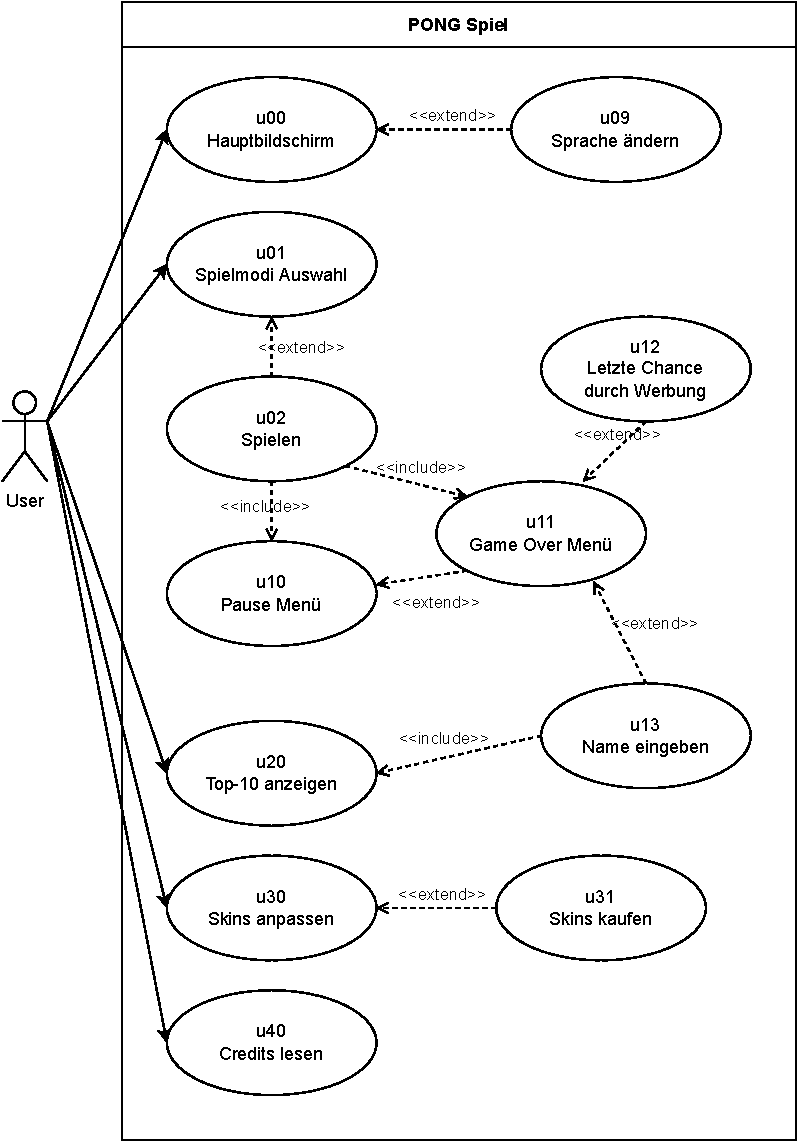
\includegraphics[width=\textwidth]{diagramme/pdf/UML-UseCase.pdf}
    \caption{Use Case Diagramm - Pong}
    \label{fig:use-case-diagram}
\end{figure}

        \subsection{Zielgruppen \& Anwender}
        Es sollen Menschen angesprochen werden, die Interesse an Mobile-Games haben und selbst welche spielen.
Der Spieleklassiker Pong wird neu interpretiert und auf Menschen aus allen Lebensbereichen ausgeweitet.
Junge \gls{spieler} werden durch modernes Design und ältere \gls{spieler} durch das nostalgische Gefühl erreicht.
\\
Die einfache Bedienung ermöglicht es dem \gls{spieler} schnell und einfach auf das Spiel zuzugreifen 
und somit Wartezeiten und Pausen schneller und angenehmer überbrücken zu können.
Angesprochen werden \gls{spieler} aller Altersklassen und jeglichen Geschlechts, die im Besitz eines Smartphones sind.
\\
Um finanzielle Barrieren zu verhindern und die Zielgruppe diesbezüglich nicht einzuschränken wird die App kostenfrei veröffentlicht.

        \subsection{IST-Zustand des Kunden}
        Pong ist ein Klassiker der Spielindustrie und wurde bereits dutzende Male neu aufgelegt.
Es gibt Desktopanwendungen, Webanwendungen und Mobile Apps. Der Großteil arbeitet aber mit dem Mehrspieler Prinzip, sodass entweder zwei Spieler gegeneinander oder ein Spieler gegen die KI spielt.

Pong als Klassiker mit moderner Grafik, als Singeplayer Spiel mit modernem In-Game Store, verschiedenen Spielmodi und verschiedenen Schwierigkeitsstufen gibt es in der Kombination noch nicht. 
        \clearpage
        \subsection{SOLL-Zustand des Kunden}
        Der letztendliche SOLL-Zustand ergibt sich final aus den \hyperref[sec:requirements]{Requirements} (Kapitel \ref{sec:requirements}).
Im Allgemeinen läst sich die Applikation wie folgt zusammenfassen:

Die App muss aus einem Startmenü, Spiel, Store, Highscore und Credits Screen bestehen.
Vom Startmnü Screen, müssen Spiel, Store, Highscore und Credits durch Buttons erreichbar sein. Auf jedem Screen muss es einen zurück Button geben.
Das Spiel muss Singleplayer und Hochkant sein.
Es muss aus zwei Spielmodi: "Classic" und "Invasion" ausgewählt werden können.
Classic und Invasion sollen aus den klassischen Elementen: Ball und Balken bestehen. 
Im Invasion Modus müssen die Kästchen eine bestimmte Anzahl von Malen getroffen werden, um zerstört zu werden.
Des Weiteren, muss es PowerUps geben.
Pro Spielmodus soll es 3 verschiedenen Schwierigkeitsstufen geben: "Easy", "Medium" und "Hard".
Unabhängig von Modus muss das Spiel jederzeit durch einen Button pausierbar sein.
Sobald der Ball unterhalb des Balkens ist, verliert der Spieler ein Leben. 
Wenn alle drei Leben aufgebraucht sind, muss es eine einmalige Chance geben, ein weiteres Leben durch das Anschauen einer Werbung zu bekommen.
Falls der Spieler einen neuen Highscore erreicht hat, muss es nach dem Spiel die Möglichkeit geben seinen Namen einzutragen.
Nach jedem Spiel muss dem Spieler sein Score und die verdienten Coins angezeigt werden.
Im Store muss man mit Coins, Skins für Ball, Ball-Schweif, Balken und Hintergründe kaufen und auswählen können.
Der Highscore Screen muss die Top 10 Scores, Namen, Spielmodi und Schwierigkeitsstufen anzeigen.
Im Credits Screen müssen die Namen von Personen, die an der Entwicklung der App gearbeitet haben und das Copyright, angezeigt werden.

    \clearpage

    \section{Produktfunktionen}\label{sec:funktionen}
        In diesem Kapitel ist der genaue Ablauf jeglicher Funktionen des Spiels beschrieben. Die einzelnen Aktivitäten ‘u‘ stehen für die jeweiligen Screens und Overlays. 
Alle mit ‘a‘ markierten Felder sind Funktionen des Spiels, die vom \gls{spieler} genutzt werden können. Alle mit ‘d‘ markierten Felder sind vom System ausgeführte Funktionen. 
Nach der Installation hat der \gls{spieler} die Möglichkeit, mit einem Klick auf das Anwendungs-Icon (zu finden in der Liste installierter Apps des Mobilgeräts) das Spiel zu starten. 
Nach maximal 5 Sekunden Ladezeit befindet sich der Spieler dann im Hauptmenü. 

Hinweis: Die Beschreibungen in diesem Kapitel (5.1) geben nur die Abläufe der jeweiligen Aktivitäten an und sind kein Indikator dafür, 
ob die genannten Funktionen Pflicht (\gls{muss}) oder optional (\gls{sollte}) sind. Alle funktionalen Anforderungen können aus der Tabelle (Kapitel 9) entnommen werden.  


        \subsection{Alle Funktionen, beschrieben aus Anwendersicht}
        

\subsubsection{Aktivität u00 - Hauptmenü}

\vspace*{1cm}

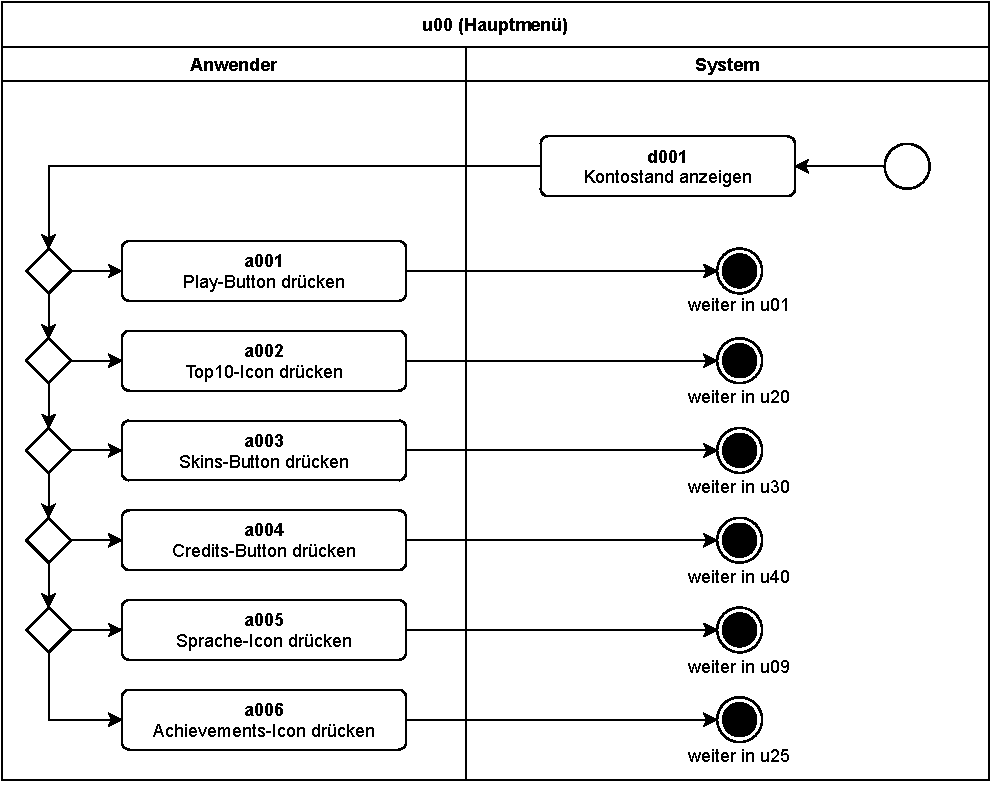
\includegraphics[width=\linewidth]{diagramme/pdf/UML-Activity-u00.pdf}
\captionof{figure}{Aktivität u00 - Hauptmenü}\label{fig:dia:mainMenu}
\vspace*{0.5cm}


Im \hyperref[fig:dia:mainMenu]{Hauptmenü} stehen dem \gls{spieler} fünf verschiedene Buttons zur Verfügung, die ihn zu anderen Screens leiten. Mit dem Play-Button gelangt man zur Spielauswahl. Über den \gls{Top10} Button kann man sich die Zehn besten Spieldurchläufe im \gls{classicMode} und \gls{invasionMode} anschauen. Im Spiel sind außerdem \gls{skin}s enthalten, die man nach Klicken des Skins-Buttons anschauen und kaufen kann. Mit dem Credits-Button gelangt man zu einem Screen, der ein paar Worte der Entwickler enthält und alle Mitwirkenden am Spiel auflistet. Über das Sprache-Icon öffnet sich ein Overlay direkt über dem \hyperref[fig:dia:mainMenu]{Hauptmenü}, dass dem \gls{spieler} die Möglichkeit gibt, die Sprache der gesamten App zu ändern. Die Standard-Sprache ist Englisch. Zuletzt gibt es noch ein weiteres Fenster für Achievements, das über das Achievements-Icon aufgerufen werden kann.


\clearpage

\subsubsection{Aktivität u01 - Spielmodus Einstellungen}

\vspace*{1cm}
   
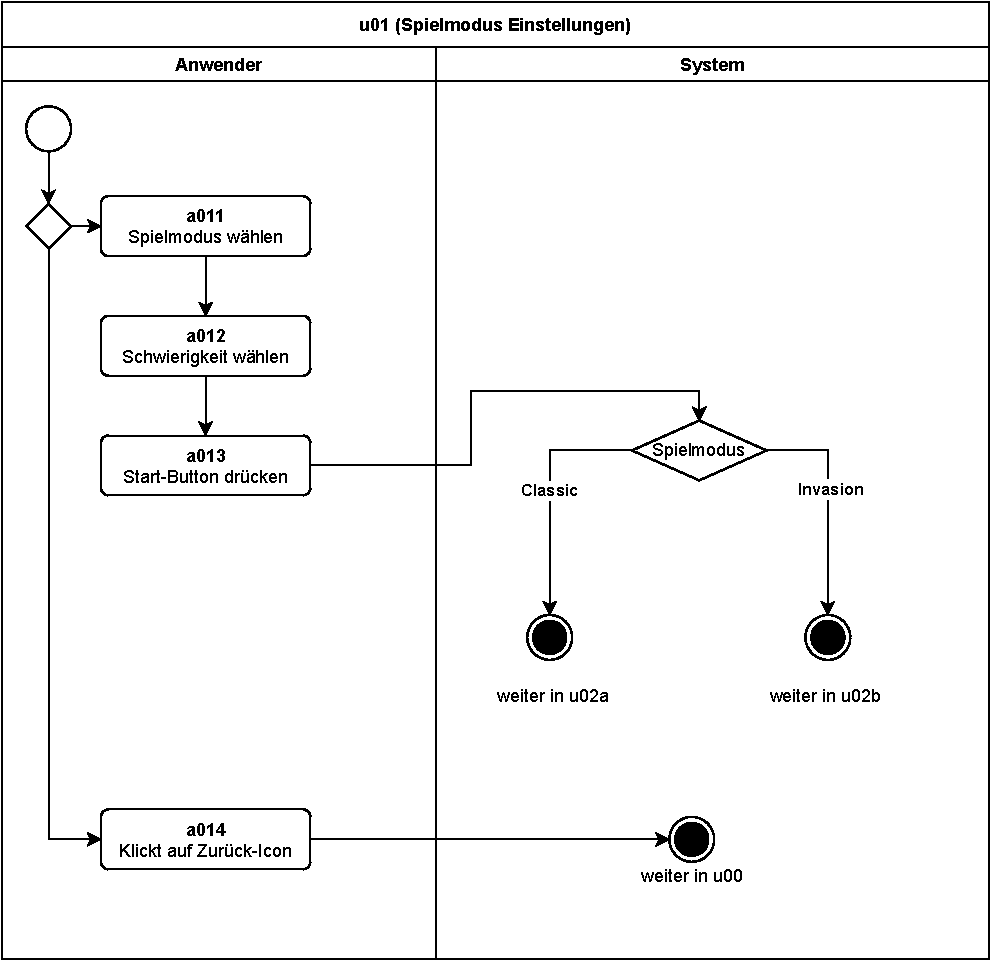
\includegraphics[width=\linewidth]{diagramme/pdf/UML-Activity-u01.pdf}
\captionof{figure}{Aktivität u01 - Spielmodus Einstellungen}\label{fig:dia:gameMode}
\vspace*{0.5cm}


Hat der \gls{spieler} den Play-Button gedrückt, so gelangt er in ein neues Fenster, dass ihm die Möglichkeit bietet, den Spielmodus (\gls{classicMode}/\gls{invasionMode}) und die Schwierigkeit (Easy, Medium, Hard) einzustellen. Drückt der \gls{spieler} dann den Start Button, wird eine neue Spielrunde mit den ausgewählten Einstellungen geladen. Über das Zurück-Icon gelangt man wieder in das \hyperref[fig:dia:mainMenu]{Hauptmenü} und die Einstellungen werden verworfen.

\clearpage

\subsubsection{Aktivität u02a - Spiel Classic}

\vspace*{1cm}

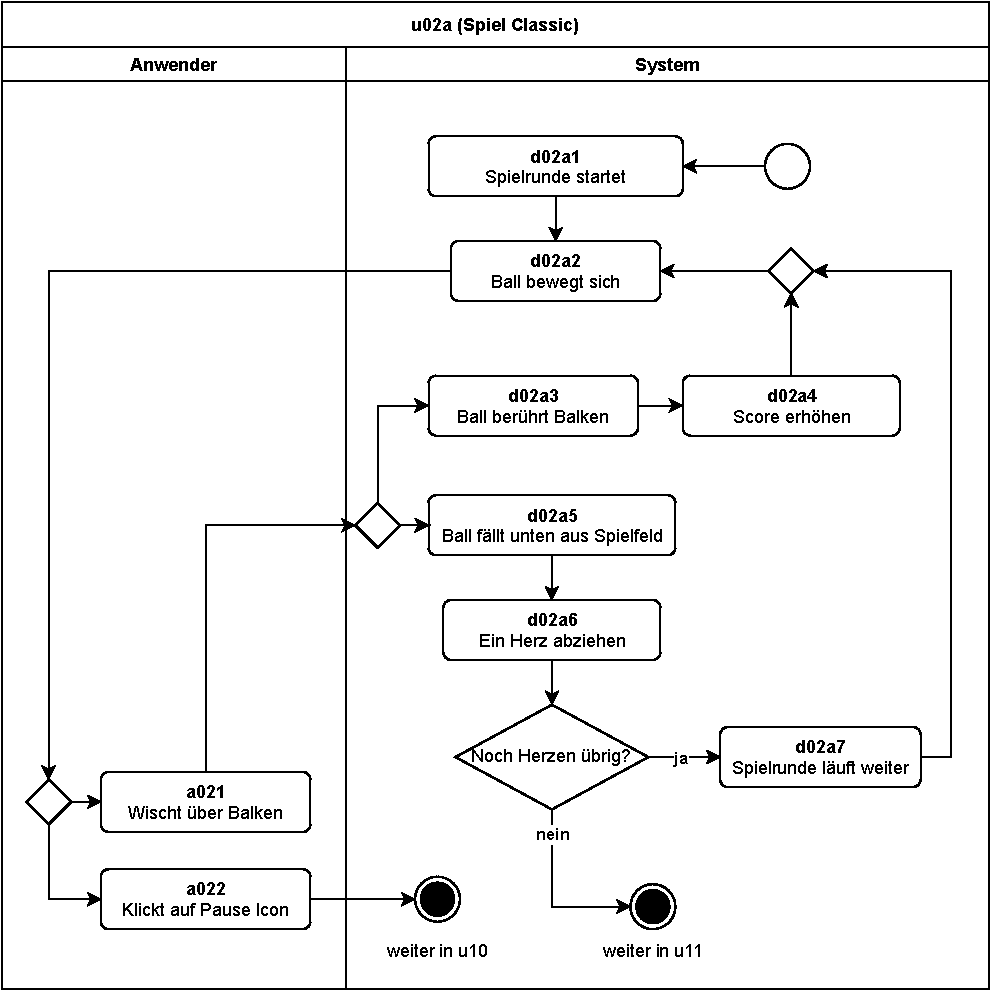
\includegraphics[width=\linewidth]{diagramme/pdf/UML-Activity-u02a.pdf}
\captionof{figure}{Aktivität u02a - Spiel Classic}\label{fig:dia:classic}
\vspace*{0.5cm}


Im \gls{classicMode} muss der \gls{spieler} den \gls{ball} mithilfe des \gls{balken} im \gls{spielfeld} halten, indem er diesen durch Wischen auf dem Screen nach links und rechts bewegt. Berührt der \gls{ball} den \gls{balken}, die Wände oder Decke des Spielfelds, so prallt er ab und ändert seine Richtung abhängig vom Auftreffwinkel. Außerdem wird der Score jedes Mal erhöht, wenn der \gls{ball} den \gls{balken} trifft.
Fällt der Ball unten aus dem \gls{spielfeld}, so verliert der Spieler ein Herz (Startet mit 3), der \gls{ball} wird wieder in die Mitte gesetzt und die Runde läuft weiter. Sollte der \gls{spieler} jedoch drei Herzen verlieren, so ist die Runde vorläufig zu Ende und der Game-Over Screen wird aufgerufen.
Der Spieler hat jedoch während der gesamten Zeit immer die Möglichkeit zu pausieren und gegebenenfalls die Runde frühzeitig zu beenden.  


\clearpage
\subsubsection{Aktivität u02b - Spiel Invasion}

\vspace*{1cm}

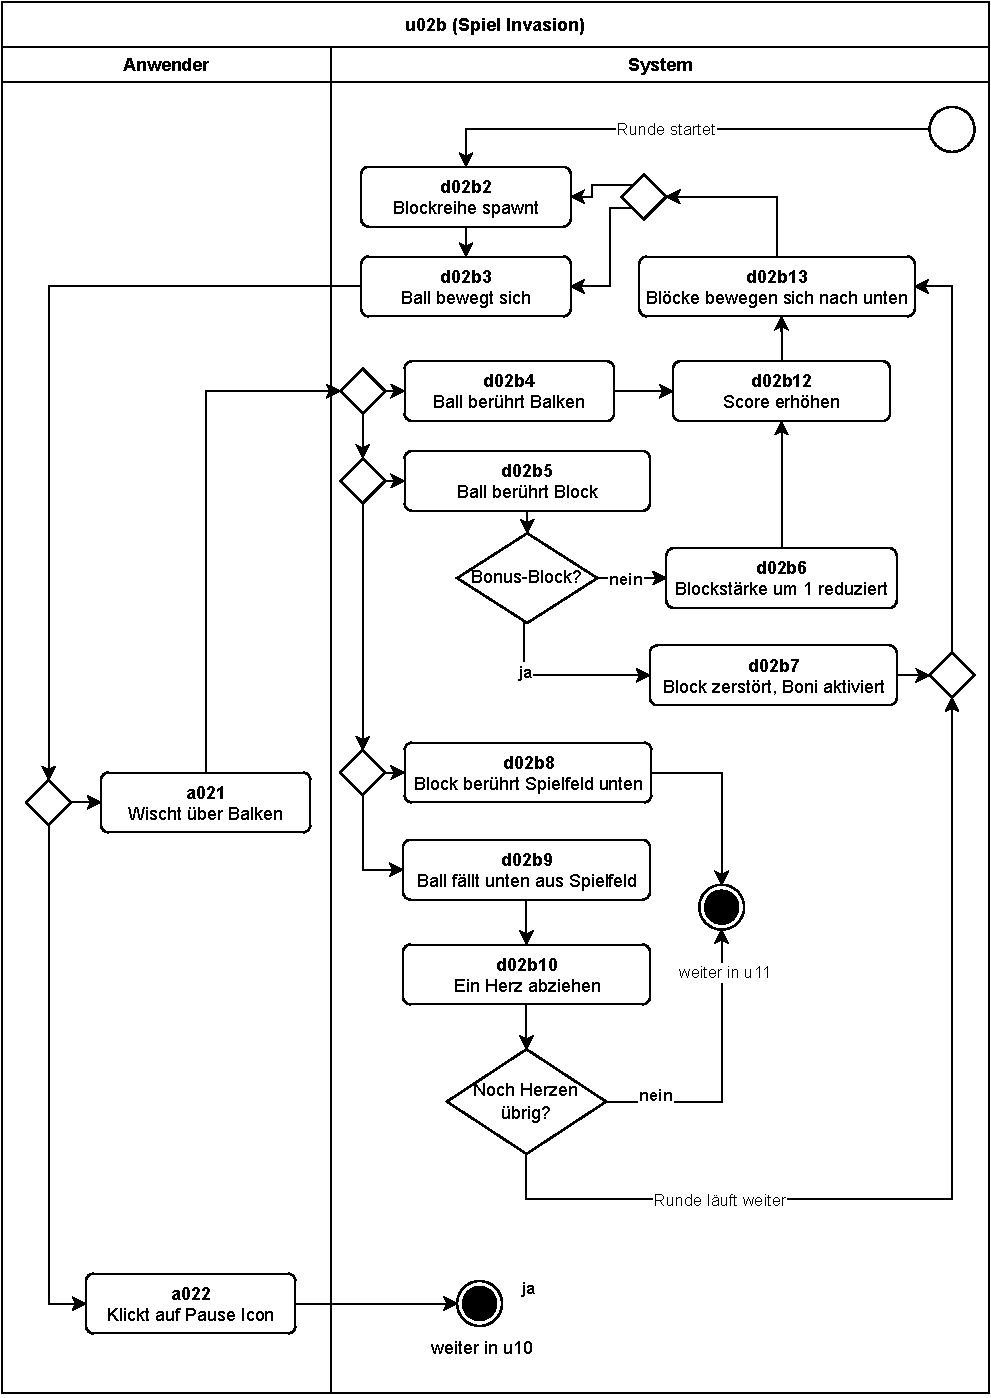
\includegraphics[width=\linewidth]{diagramme/pdf/UML-Activity-u02b.pdf}
\captionof{figure}{Aktivität u02b - Spiel Invasion}\label{fig:dia:invasion}
\vspace*{0.5cm}


Der \gls{invasionMode} ist eine Erweiterung zum \gls{classicMode}. Ab Rundenstart spawnt periodisch eine Reihe an Blöcken verschiedener Stärke und vereinzelt mit Boni für den \gls{spieler}. Diese Blöcke müssen mehrmals (abhängig von der Stärke des Blocks) vom \gls{ball} getroffen werden, um sie zu zerstören. Zerstört der Spieler einen Bonus-\gls{block}, so erhält der \gls{ball} (oder der \gls{spieler}) für kurze Zeit eine besondere Eigenschaft. (Siehe 9.2.1). 
Alle anderen Spielabläufe des \gls{invasionMode} sind identisch zu dem des \gls{classicMode} (5.1.3).


\clearpage

\subsubsection{Aktivität u09 - Sprachauswahl}

\vspace*{1cm}

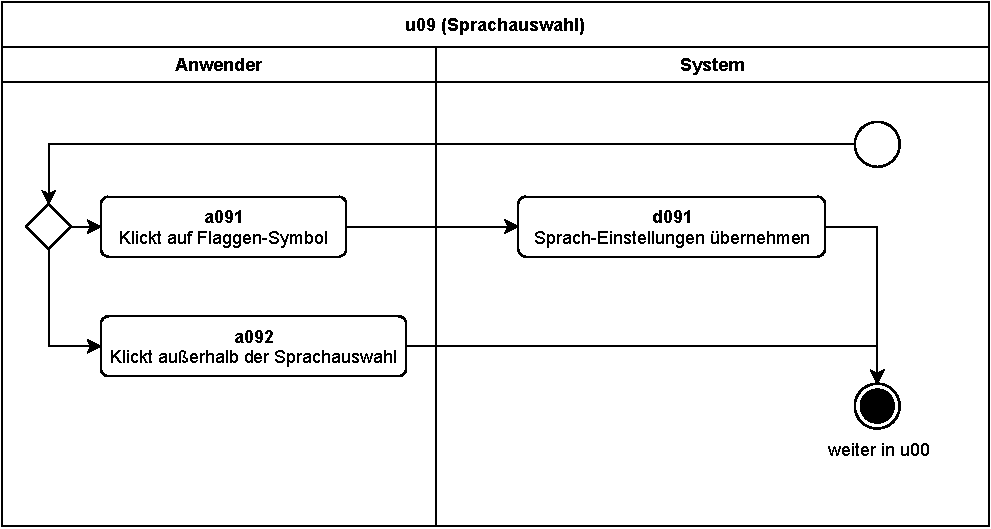
\includegraphics[width=\linewidth]{diagramme/pdf/UML-Activity-u09.pdf}
\captionof{figure}{Aktivität u09 - Sprachauswahl}\label{fig:dia:language}
\vspace*{0.5cm}



Wurde das Sprache-Icon im Hauptmenü gedrückt, öffnet sich ein Overlay. Darin hat der \gls{spieler} die Möglichkeit die Sprache des Spiels zu ändern, indem er auf eine der verfügbaren Flaggen klickt. Die Standardeinstellung der Sprache ist Englisch. Durch das Klicken außerhalb der Sprachauswahl kommt der \gls{spieler} wieder in das \hyperref[fig:dia:mainMenu]{Hauptmenü} zurück.

\clearpage

\subsubsection{Aktivität u09 - Achievements}

\vspace*{1cm}

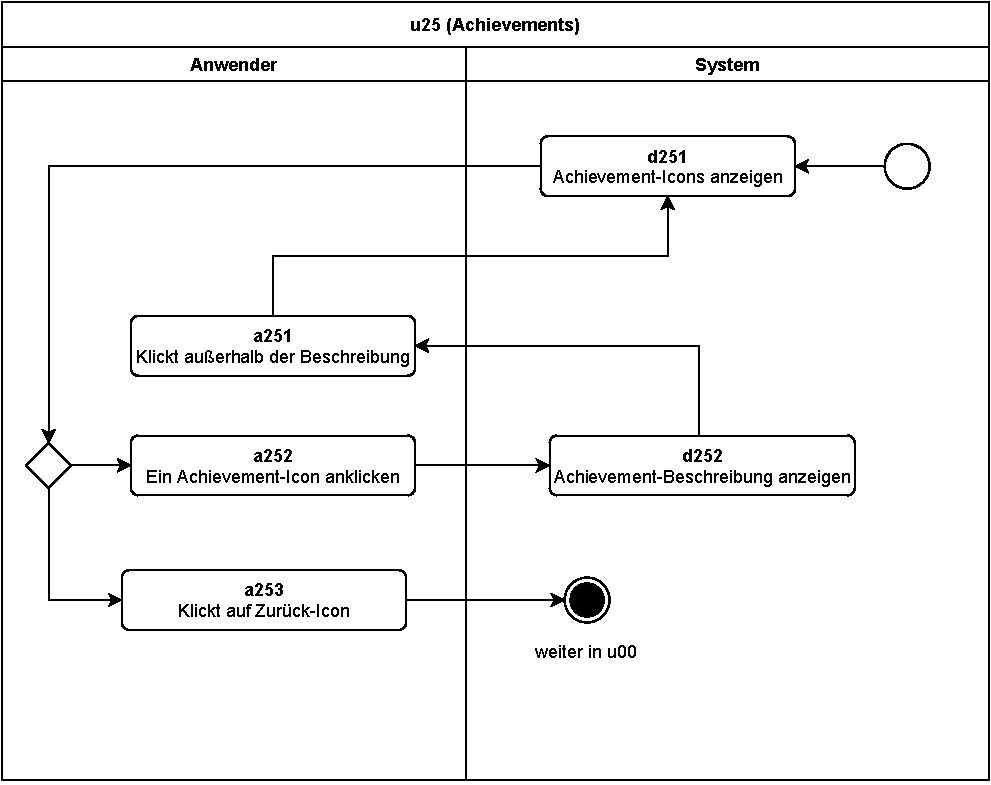
\includegraphics[width=\linewidth]{diagramme/pdf/UML-Activity-u25.pdf}
\captionof{figure}{Aktivität u25 - Achievements}\label{fig:dia:achievements}
\vspace*{0.5cm}

Über das Achievements-Icon gelangt der \gls{spieler} auf einen Screen, der alle seine bisher erreichten Achievements anzeigt (Noch nicht erreichte sind ausgegraut sein). Wird auf eines der Icons geklickt, so öffnet sich ein Overlay und der Spieler kann die Beschreibung des jeweiligen Achievements nachlesen. Durch das Klicken des Zurück-Icons gelangt der Spieler dann wieder in das \hyperref[fig:dia:mainMenu]{Hauptmenü}. 

\clearpage

\subsubsection{Aktivität u10 - Pause Menü}


\vspace*{1cm}

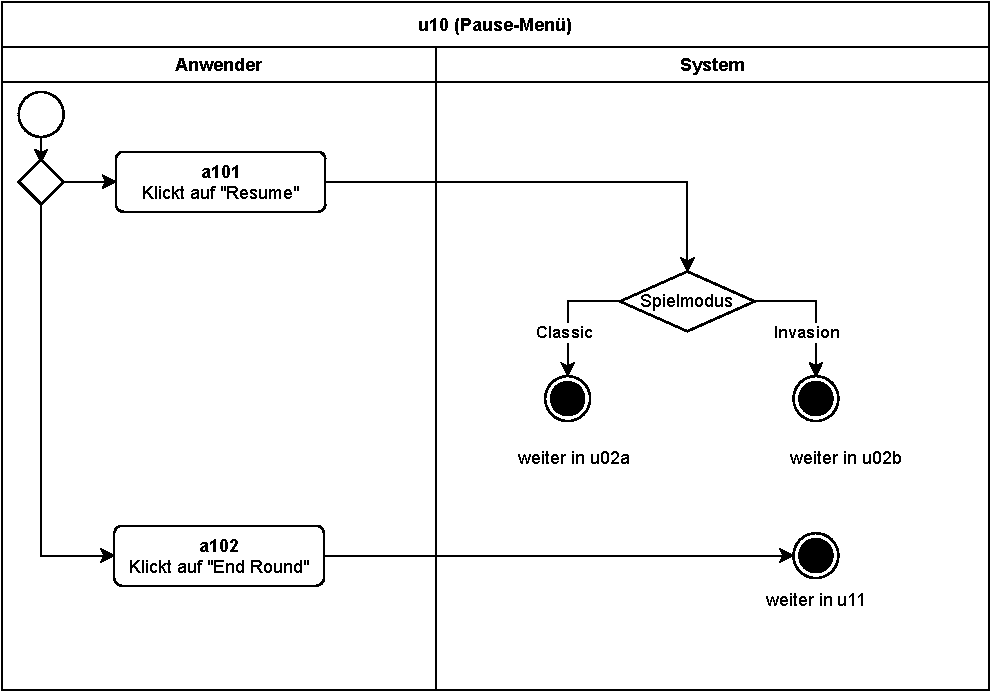
\includegraphics[width=\linewidth]{diagramme/pdf/UML-Activity-u10.pdf}
\captionof{figure}{Aktivität u10 - Pause Menü}\label{fig:dia:pause}
\vspace*{0.5cm}


Während einer aktiven Spielrunde hat der \gls{spieler} die Möglichkeit zu pausieren. Dann wird das Spiel angehalten und ein Overlay öffnet sich. Darin kann der Spieler entweder den Resume Button klicken, um die jeweilige Runde fortzusetzen, oder auf End Round klicken, um die Runde frühzeitig zu beenden.

\clearpage

\subsubsection{Aktivität u11 - Game-Over-Menü}

\vspace*{1cm}

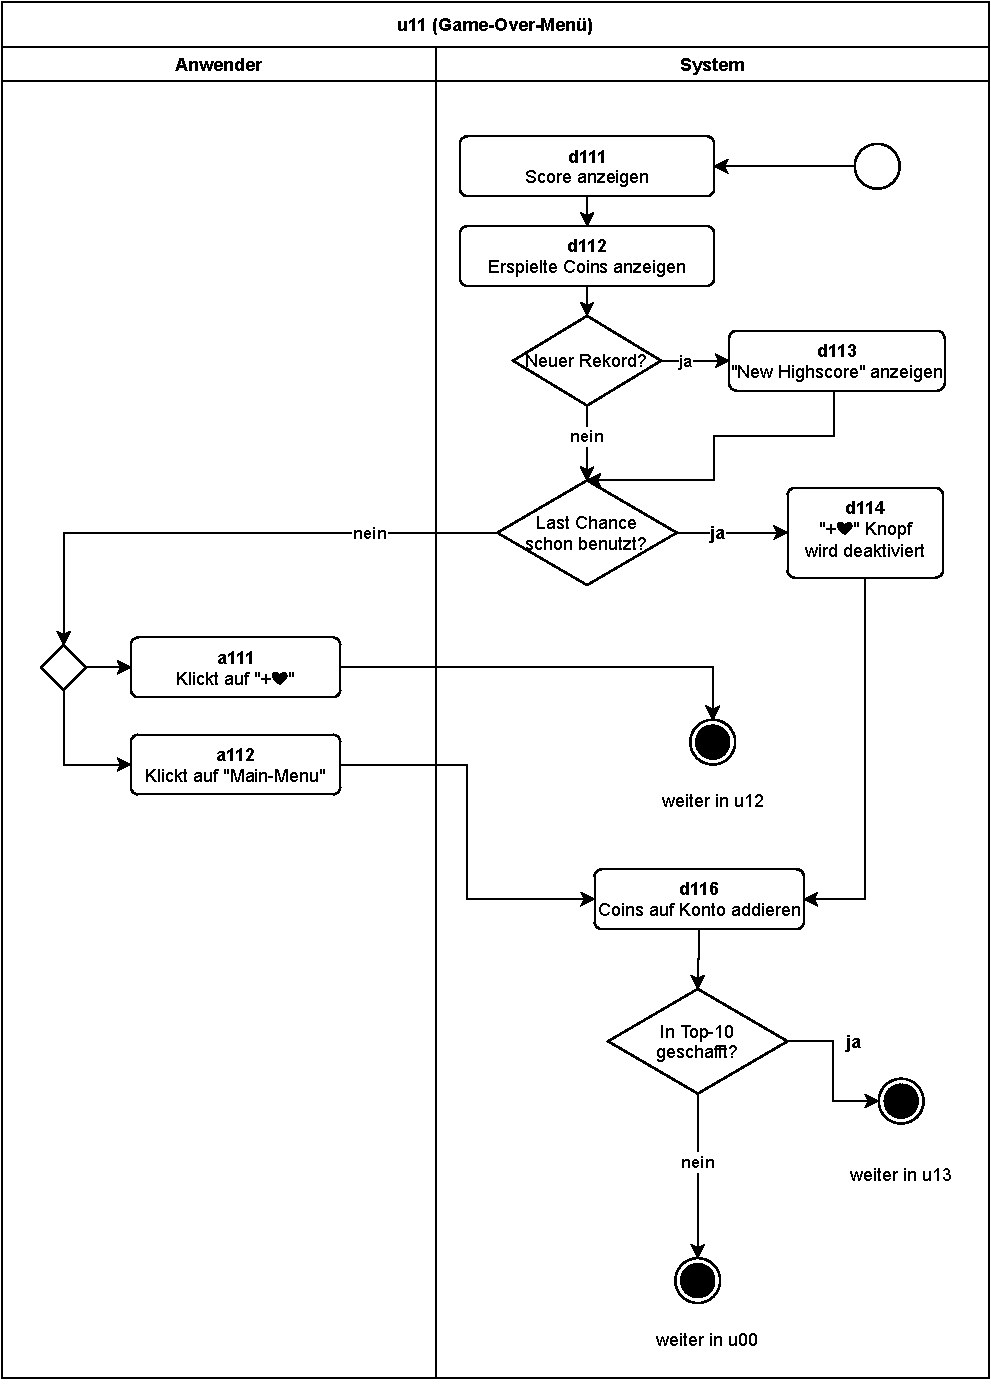
\includegraphics[width=\linewidth]{diagramme/pdf/UML-Activity-u11.pdf}
\captionof{figure}{Aktivität u11 - Game-Over-Menü}\label{fig:dia:gameOver}
\vspace*{0.5cm}


Hat der \gls{spieler} alle seine Herzen verloren, oder die Runde im Pause Menü frühzeitig beendet, so kommt er automatisch in das Game-Over Menü. Hier sieht er den bisher erreichten Score und die erspielten Coins. Hat er in der Runde einen höheren Score erreicht als der erste Platz in der \gls{Top10} Liste, bekommt der \gls{spieler} die Nachricht „new Highscore“ auf dem Screen angezeigt. Hat der \gls{spieler} noch keine „last Chance“ genutzt, so bietet ihm das System einmalig die Möglichkeit, einen Werbeclip zu schauen, um nochmal ein Herz zu erhalten und die Runde fortzusetzen. Verliert der \gls{spieler} auch dieses Herz ist die Runde endgültig zu Ende. Danach werden die erspielten Coins automatisch auf das Spiel-Konto addiert und das System prüft, ob der Score des Spielers hoch genug ist um in die \gls{Top10} zu kommen. Ist dies der Fall, so wird eine Namenseingabe angezeigt, in der der \gls{spieler} seinen Namen eingeben kann. Hat der \gls{spieler} keine \gls{Top10} Platzierung erreicht, wird das \hyperref[fig:dia:mainMenu]{Hauptmenü} geöffnet.
\clearpage

\subsubsection{Aktivität u12 - Werbung}

\vspace*{1cm}

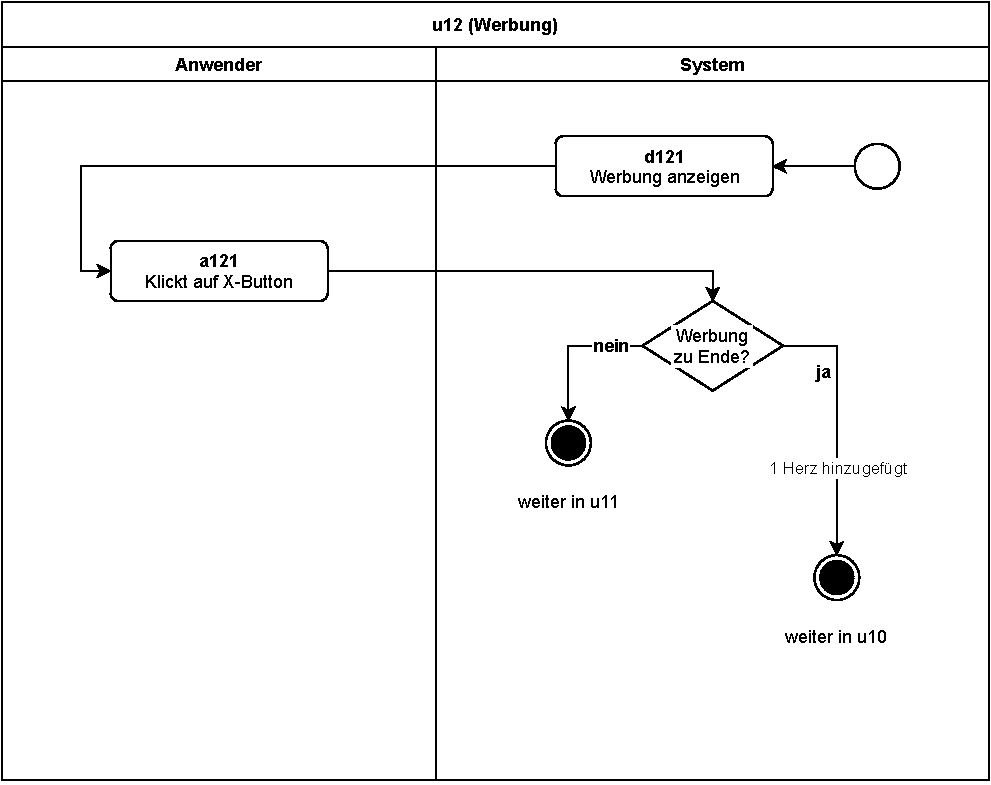
\includegraphics[width=\linewidth]{diagramme/pdf/UML-Activity-u12.pdf}
\captionof{figure}{Aktivität u12 - Werbung}\label{fig:dia:ads}
\vspace*{0.5cm}

Entscheidet sich der \gls{spieler} Werbung anzuschauen, so hat er die Möglichkeit, diese über den „X“ Button wieder zu schließen. Ist die Werbung zu diesem Zeitpunkt noch nicht vollständig durchgelaufen, so wird der \gls{spieler} wieder in das Game-Over Menü weitergeleitet. Hat er sich die Werbung jedoch vollständig angeschaut, so erhält er ein extra Herz und wird zum Pause Menü weitergeleitet, sodass die Runde fortgesetzt werden kann.

\clearpage

\subsubsection{Aktivität u13 - Namenseingabe}

\vspace*{1cm}

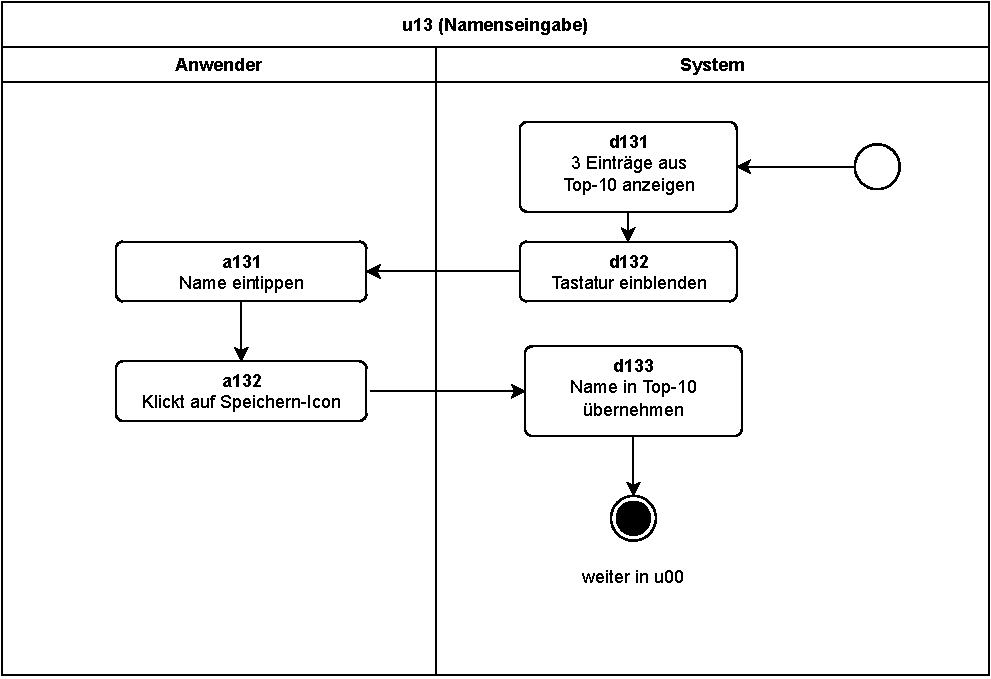
\includegraphics[width=\linewidth]{diagramme/pdf/UML-Activity-u13.pdf}
\captionof{figure}{Aktivität u13 - Namenseingabe}\label{fig:dia:highscore}
\vspace*{0.5cm}

Hat der \gls{spieler} nach der Runde eine \gls{Top10} Platzierung erreicht, so wird die Namenseingabe angeboten. Es werden, sofern vorhanden, drei Einträge der Platzierungen genau vor dem des erreichten Scores angezeigt. Unterhalb dieser Anzeige wird die Tastatur
eingeblendet und der \gls{spieler} hat so die Möglichkeit seinen Namen einzutippen und anschließend durch den Klick auf das Speichern-Icon seinen Namen in den \gls{Top10} zu sichern. Danach wird der \gls{spieler} wieder in das \hyperref[fig:dia:mainMenu]{Hauptmenü} geleitet.

\clearpage

\subsubsection{Aktivität u20 - Top-10 Liste}

\vspace*{1cm}

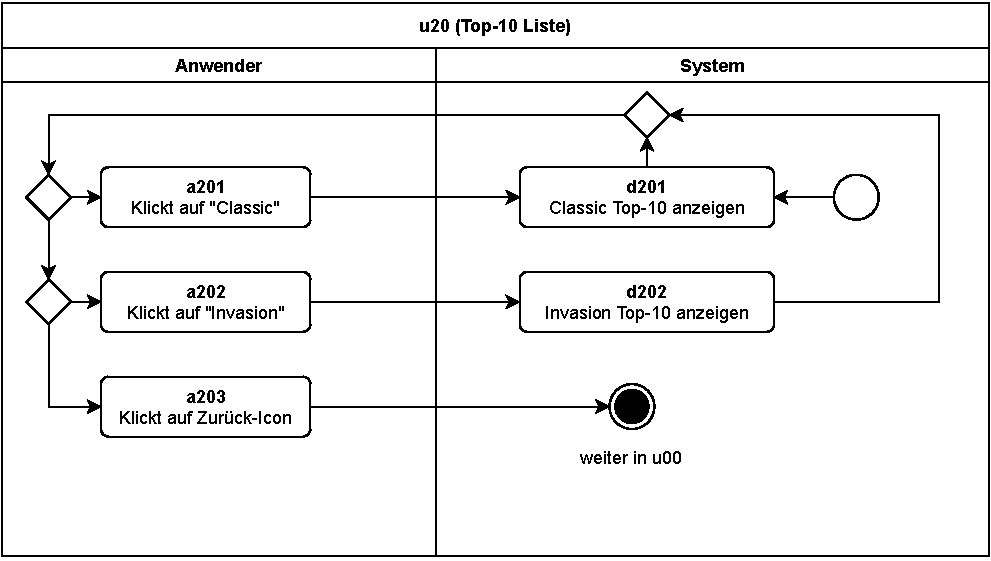
\includegraphics[width=\linewidth]{diagramme/pdf/UML-Activity-u20.pdf}
\captionof{figure}{Aktivität u20 - Top-10 Liste}\label{fig:dia:top10}
\vspace*{0.5cm}

Klickt der \gls{spieler} im \hyperref[fig:dia:mainMenu]{Hauptmenü} auf den \gls{Top10} Button, so werden ihm standardmäßig die 10 höchsten Scores im \gls{classicMode} in Listenform angezeigt. Durch einen klick auf den Invasion-Button ändert sich die Liste und zeigt dann die 10 höchsten Scores im \gls{invasionMode}. Analog dazu führt der Classic-Button zur Top-10 Liste des \gls{classicMode} zurück.
Über das Zurück-Icon gelangt der \gls{spieler} wieder in das \hyperref[fig:dia:mainMenu]{Hauptmenü}.

\clearpage

\subsubsection{Aktivität u30 - Skin-Auswahl}

\vspace*{1cm}

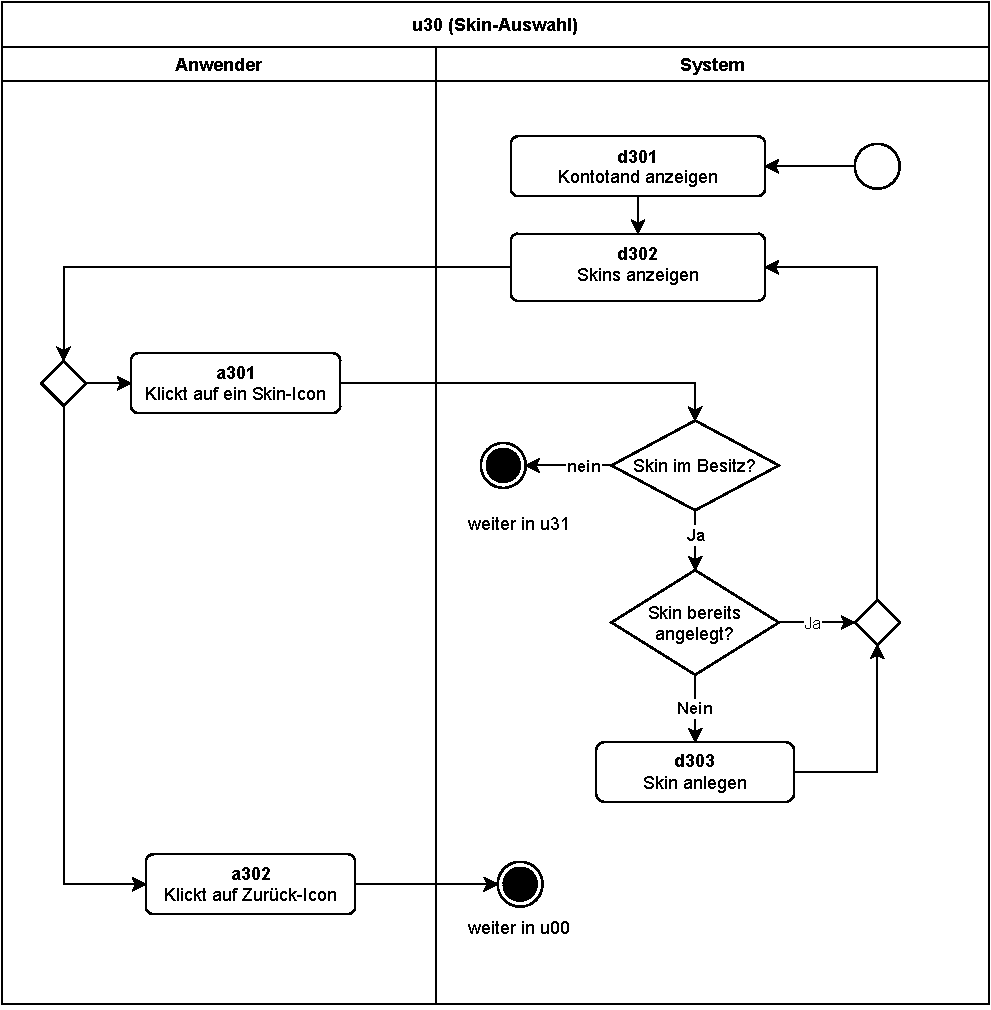
\includegraphics[width=\linewidth]{diagramme/pdf/UML-Activity-u30.pdf}
\captionof{figure}{Aktivität u30 - Skin-Auswahl}\label{fig:dia:skins}
\vspace*{0.5cm}

Klickt der Spieler auf den Skins-Button, so gelangt er auf einen Screen, der ihm alle im Spiel verfügbaren \gls{skin}s des \gls{ball}s, des \gls{tail}s und des Hintergrunds anzeigt. Zusätzlich sieht er hier auch nochmal seinen aktuellen Kontostand. Durch Klicken eines Skin-Icons wird ein Overlay geöffnet, das dem \gls{spieler} die Möglichkeit bietet, den \gls{skin} zu kaufen oder anzulegen. Ist der ausgewählte \gls{skin} bereits angelegt, so wird das Overlay geschlossen und der Spieler kehrt zu der Anzeige aller \gls{skin}s zurück.
\clearpage

\subsubsection{Aktivität u31 - Skin kauf}

\vspace*{1cm}

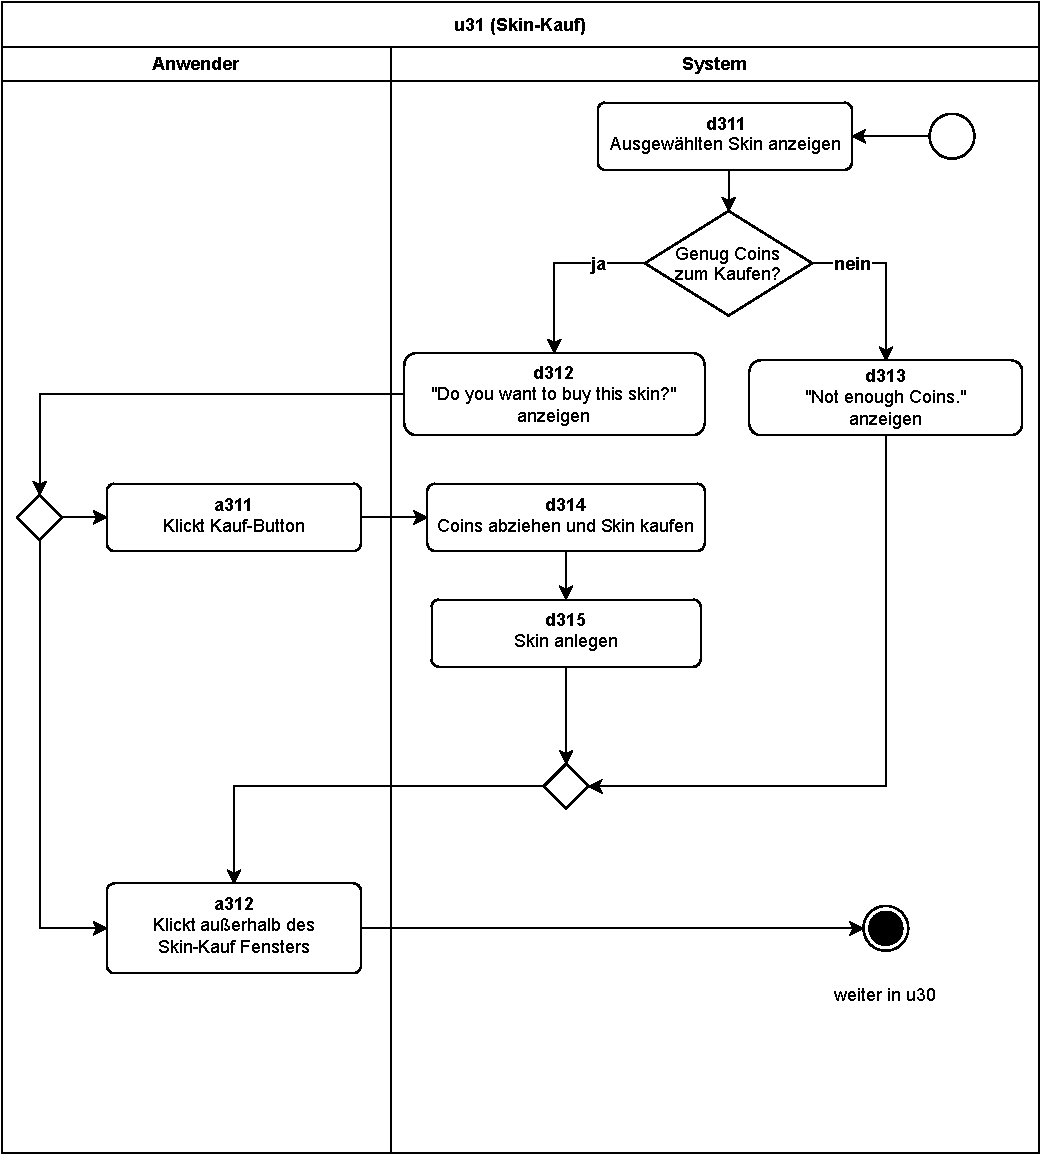
\includegraphics[width=\linewidth]{diagramme/pdf/UML-Activity-u31.pdf}
\captionof{figure}{Aktivität u31 - Skin kauf}\label{fig:dia:skinPurchase}
\vspace*{0.5cm}

Hat der \gls{spieler} einen \gls{skin} ausgewählt, so wird ein Overlay geöffnet. Ist der \gls{skin} noch nicht in seinem Besitz, so wird vom System geprüft, ob genügend Coins für den Kauf des \gls{skin}s vorhanden sind. Ist dies der Fall, so wird die Nachricht „Do you want to buy this skin?“ angezeigt. Entscheidet sich dann der \gls{spieler} disen zu kaufen, so werden die benötigten Coins von seinem Konto abgezogen, der \gls{skin} freigeschaltet und direkt angelegt. 
Fehlen dem \gls{spieler} noch Coins für den \gls{skin}, so zeigt das System die Nachricht „Not enough Coins“ an. Mit einem Klick außerhalb des Overlays kommt der \gls{spieler} dann wieder zurück auf die Anzeige aller \gls{skin}s.

\clearpage

\subsubsection{Aktivität u40 -Credits}

\vspace*{1cm}

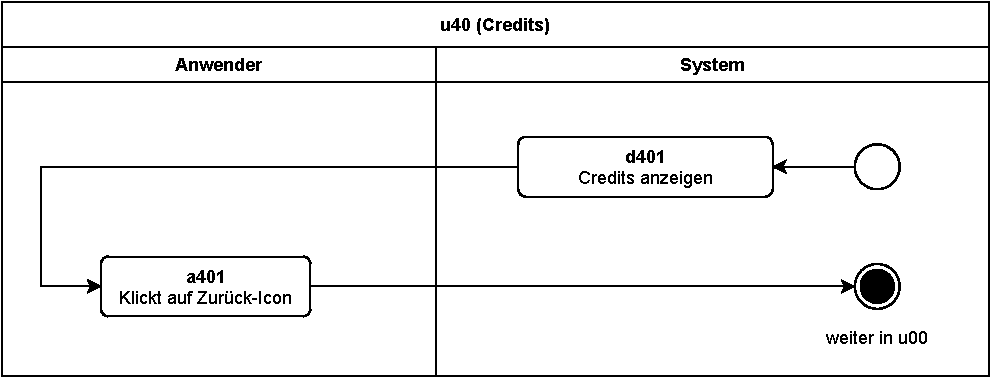
\includegraphics[width=\linewidth]{diagramme/pdf/UML-Activity-u40.pdf}
\captionof{figure}{Aktivität u40 -Credits}\label{fig:dia:credits}
\vspace*{0.5cm}

Bei einem Klick auf den Credits-Button muss das System dem \gls{spieler} die Credits anzeigen. 
Dieser enthält paar Worte der Entwickler und listet alle Mitwirkenden am Spiel auf. 
Der \gls{spieler} hat die Möglichkeit den Credits Screen durch einen Klick auf das Zurück-Icon zu verlassen und das \hyperref[fig:dia:mainMenu]{Hauptmenü} zu erreichen.

\clearpage






        \subsection{Eingabe/Ausgabe}
        Im Folgenden werden Mockups präsentiert, welche das Design und die Benutzeroberfläche der PONG App darstellen. Kleinere Änderungen an Design und der Benutzeroberfläche während des Entwicklungsprozesses sind möglich.

\subsubsection{Icon Legende}
\vspace*{0.5cm}

\begin{center}
    \begin{tabular}{ll}
        
\includegraphics[width=1.5em,height=1.5em]{diagramme/assets/Media-Play-256.png} & Start / Fortsetzen \\
        
\includegraphics[width=1.5em,height=1.5em]{diagramme/assets/Media-Pause-256.png} & Pause \\
        
\includegraphics[width=1.5em,height=1.5em]{diagramme/assets/Close-256.png} & Beenden\\
        
\includegraphics[width=1.5em,height=1.5em]{diagramme/assets/Arrow-Left-05-256.png} & Zurück \\
        
\includegraphics[width=1.5em,height=1.5em]{diagramme/assets/Floppy-256.png} & Speichern und Fortfahren \\
        
\includegraphics[width=1.5em,height=1.5em]{diagramme/assets/Money-Coin-02-WF-256.png} & Coins / Kontostand \\
        
\includegraphics[width=1.5em,height=1.5em]{diagramme/assets/Heart-256.png} & Symbolisiert ein Leben \\
        
\includegraphics[width=1.5em,height=1.5em]{diagramme/assets/Globe-256.png} & Sprachauswahl \\
        
\includegraphics[width=1.5em,height=1.5em]{diagramme/assets/Shirt-256.png} & Allgemeines Symbol für Skins \\
        
\includegraphics[width=1.5em,height=1.5em]{diagramme/assets/list.png} & Top-10 Liste \\
        
\includegraphics[width=1.5em,height=1.5em]{diagramme/assets/Trophy-256.png} & Achivements \\
        
\includegraphics[width=1.5em,height=1.5em]{diagramme/assets/Bomb-256.png} & Beispiel für Powerup \\    
        
\includegraphics[width=1.5em,height=1.5em]{diagramme/assets/Lock-256.png} & Item gesperrt / nicht im Besitz
    \end{tabular}
\end{center}
\setlength{\extrarowheight}{0.5em}

\clearpage

\subsubsection{Dialog u00 - Hauptmenü}


\begin{wrapfigure}{l}{0.5\textwidth}
    \begin{center}
    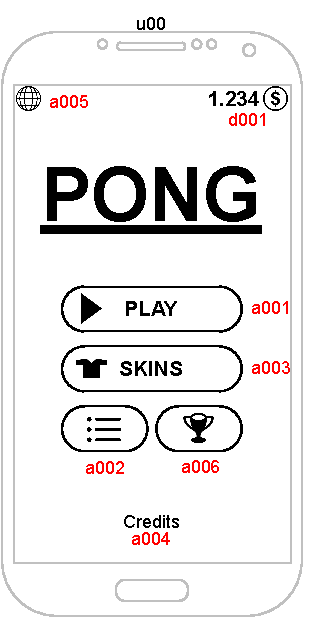
\includegraphics{diagramme/pdf/Mockup-u00.pdf}
    \end{center}
    \caption{Dialog u00 - Hauptmenü}
\end{wrapfigure}

Das Hauptmenü dient dem \gls{spieler} als Ausgangspunkt. Von hier aus kann es möglich sein die Sprache zu ändern (a005) und die persönlichen Achivements einzusehen (a006). 
Es muss hingegen möglich sein, die Anzahl der Coins einzusehen (d001), zur Spielauswahl zu gelangen (a001), zum InGame Store zu gelangen (a003), die TopTen Liste einzusehen (a002) und die Credits  zu öffnen (a004).

\clearpage

\subsubsection{Dialog u01 - Spielmodus Einstellungen}

\begin{wrapfigure}{l}{0.5\textwidth}
    \begin{center}
    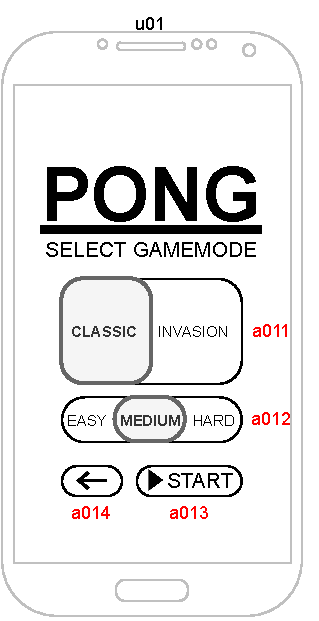
\includegraphics{diagramme/pdf/Mockup-u01.pdf}
    \end{center}
    \caption{Dialog u01 - Spielmodus Einstellungen}
\end{wrapfigure}

Möchte der \gls{spieler} ein Spiel starten, so kann er zunächst zwischen den Spielmodi "Classic" und "Invasion" wählen (a012). Der \gls{spieler} muss die Möglichkeit haben, von einem aus drei Schwierigkeitsstufen zu wählen (a011).
Außerdem muss es dem \gls{spieler} möglich sein, zurück zum Hauptmenü zu kommen (a015).
\clearpage

\subsubsection{Dialog u02a - Spiel Classic}

\begin{wrapfigure}{l}{0.5\textwidth}
    \begin{center}
    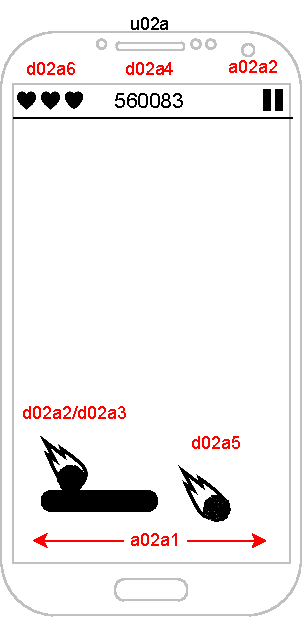
\includegraphics{diagramme/pdf/Mockup-u02a.pdf}
\end{center}
    \caption{Dialog u02a - Spiel Classic}
\end{wrapfigure}

Der Screen "Spiel Classic" muss neben dem beweglichen \gls{balken} (a02a1) und dem \gls{ball} die aktuelle Lebensanzeige und die aktuelle Punktzahl anzeigen.
Außerdem muss in der rechten oberen Ecke ein Pause-Button die möglichkeit bieten das aktuelle Spiel zu pausieren (a02a2).
Verpasst der Spieler den Ball mit dem Balken und der Ball berührt den unteren Bildschirmrand, so ist das Spiel verloren (d02a5).
\vspace*{1cm}
\clearpage

\subsubsection{Dialog u02b - Spiel Invasion}

\begin{wrapfigure}{l}{0.5\textwidth}
    \begin{center}
    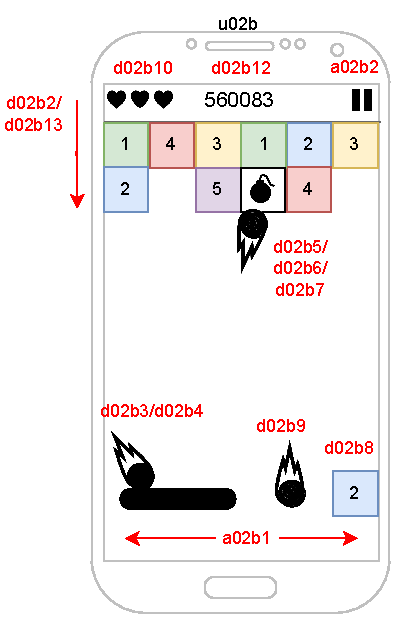
\includegraphics{diagramme/pdf/Mockup-u02b.pdf}
\end{center}
    \caption{Dialog u02b - Spiel Invasion}
\end{wrapfigure}

Bei dem optionalen Spielmodus "Invasion" können neben den UI Elementen aus u02a noch die Spielmodus spezifischen Elemente auftauchen. 
Hierbei handelt es sich um Blöcke, welche zerstört werden können. Hierbei können die Blöcke unterschiedliche Stärken besitzen. 
Die Stärke repräsentiert hierbei die Anzahl an \gls{ball}berührungen, die es benötigt um einen Block zu zerstören. Außerdem können Power-Up Blöcke
erscheinen, welche dem \gls{spieler} temporäre Vorteile verschaffen. Berührt rin Block den unteren Rand des Bildschirms, so ist das Spiel ebenfalls beendet (d02b8).
\clearpage

\subsubsection{Dialog u09 - Sprachauswahl}

\begin{wrapfigure}{l}{0.5\textwidth}
    \begin{center}
    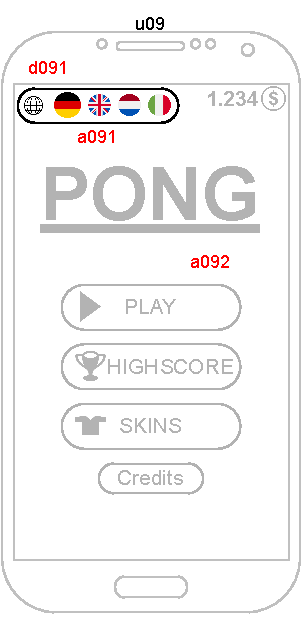
\includegraphics{diagramme/pdf/Mockup-u09.pdf}
\end{center}
    \caption{Dialog u09 - Sprachauswahl}
\end{wrapfigure}

Bei der optionalen Sprachauswahl kann der \gls{spieler} zwischen verschiedenen Sprachen wählen und somit den im Spiel angezeigten Text entsperchend der Auswahl ünersetzen lassen.
\clearpage

\subsubsection{Dialog u10 - Pause Menü}

\begin{wrapfigure}{l}{0.5\textwidth}
    \begin{center}
    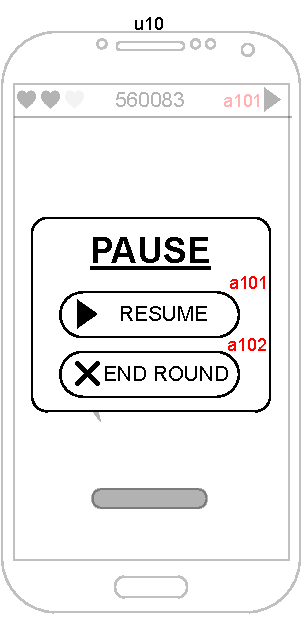
\includegraphics{diagramme/pdf/Mockup-u10.pdf}
\end{center}
    \caption{Dialog u10 - Pause Menü}
\end{wrapfigure}

Das Pause-Menü muss dem \gls{spieler} die Optionen geben, entweder das Spiel zu beenden (a102), oder das Spiel fortzusetzen (a101).

\clearpage

\subsubsection{Dialog u11 - Game-Over-Menü}

\begin{wrapfigure}{l}{0.5\textwidth}
    \begin{center}
    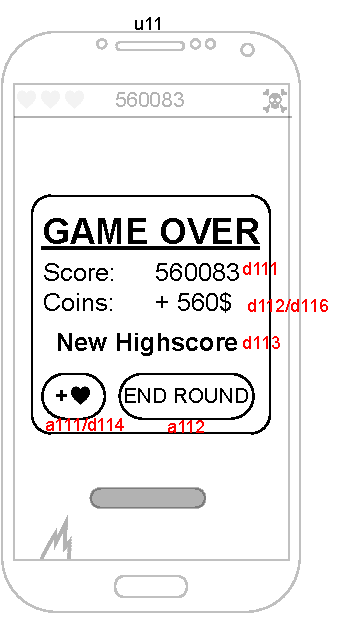
\includegraphics{diagramme/pdf/Mockup-u11.pdf}
    \end{center}
    \caption{Dialog u11 - Game-Over-Menü}
\end{wrapfigure}

Hat der \gls{spieler} keine Herzen mehr, so muss der Game-Over Screen angezeigt werden. Dieser bietet beim ersten Mal nach jeder Spielrunde die Möglichkeit ein letzte Chance zu bekommen (a111).
Außerdem muss der erreichte Score (d111) und die erspielten Coins (d112) angezeigt werden.
Der \gls{spieler} muss mit einem Klick auf "End Round" (a112) zurück ins Hauptmenü geleitet werden.
\clearpage

\subsubsection{Dialog u12 - Werbung}

\begin{wrapfigure}{l}{0.5\textwidth}
    \begin{center}
    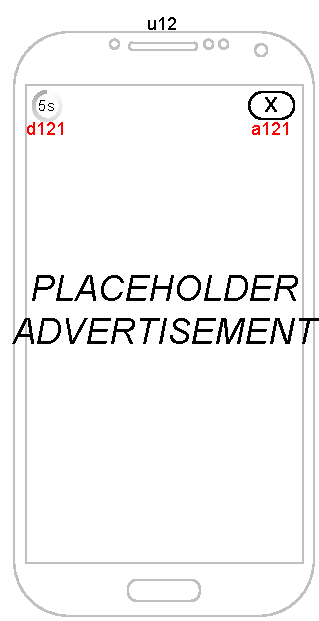
\includegraphics{diagramme/pdf/Mockup-u12.pdf}
    \end{center}
    \caption{Dialog u12 - Werbung}
\end{wrapfigure}

Entscheidet sich der \gls{spieler} dazu, ein weiteres Leben durch einen Werbeclip zu bekommen, so muss eine Platzhalter-Werbung angezeigt werden.
Nach Ablauf der Werbung, muss der \gls{spieler} diese beenden (a121) und kann weiter spielen.
\clearpage

\subsubsection{Dialog u13 - Namenseingabe}

\begin{wrapfigure}{l}{0.5\textwidth}
    \begin{center}
    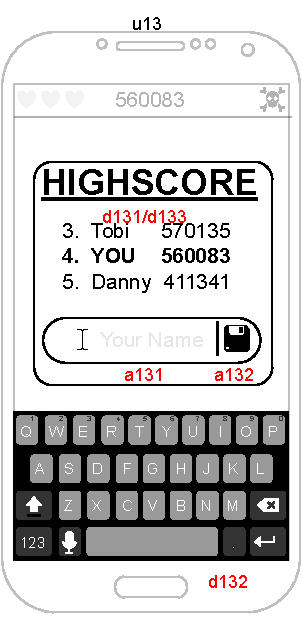
\includegraphics{diagramme/pdf/Mockup-u13.pdf}
\end{center}
    \caption{Dialog u13 - Namenseingabe}
\end{wrapfigure}

Hat der \gls{spieler} eine TopTen Platzierung erspielt, so muss ihm seine Position in der TopTen Liste nach Ablauf der Spielrunde angezeigt werden.
Neben dem gerade erspieleten Score müssen ebenfalls die zwei nächsten Scores angezeigt werden.
Der \gls{spieler} muss dann die Möglichkeit haben, seinen Namen einzutragen (a131) und sich mit einem Klick auf den Speichern Button (a132) in der TopTen Liste abzuspeichern.
\clearpage

\subsubsection{Dialog u20 - Top-10 Liste}

\begin{wrapfigure}{l}{0.5\textwidth}
    \begin{center}
    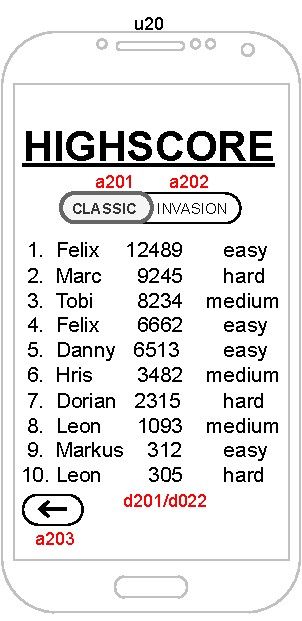
\includegraphics{diagramme/pdf/Mockup-u20.pdf}
\end{center}
    \caption{Dialog u20 - Top-10 Liste}
\end{wrapfigure}

Die TopTen Liste muss die zehn besten Scores präsentieren und es kann für jeden Spielmodus eine einzelne Liste geben. 
Neben der Platzierung, dem Namen und der Punkte, muss ebenfalls der Spielmodus angezeigt werden, mit welchem die Platzierung erreicht wurde.
\clearpage

\subsubsection{Dialog u25 - Achivements}

\begin{figure}[h!]
    \begin{center}
        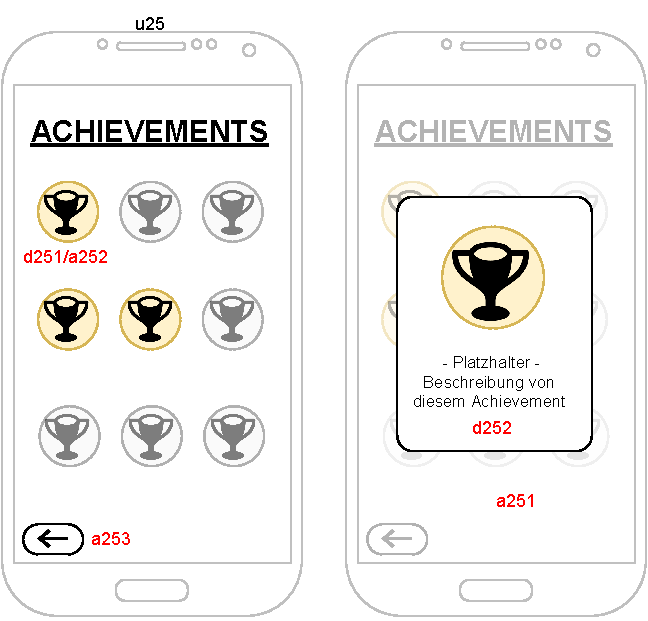
\includegraphics{diagramme/pdf/Mockup-u25.pdf}
    \end{center}
    \caption{Dialog u25 - Achivements}
\end{figure}

Auf dem Achivements Bildschirm sollen alle erreichbaren \gls{achievements} als Symbol dargestellt werden. Noch nicht freigeschaltete \gls{achievements} sollen  ausgegraut dargestellt werden. Klickt der \gls{spieler} auf ein Achivementsymbol, soll die dazugehörige Beschreibung angezeugt werden. Ein Klick außerhalb der Beschreibung soll diese wieder schließen. Dem \gls{spieler} soll es möglich sein, durch einen Klick auf den Zurück-Pfeil wieder ins Hauptmenü zu gelangen.
\clearpage

\subsubsection{Dialog u30 - Skin Auswahl}

\begin{wrapfigure}{l}{0.5\textwidth}
    \begin{center}
    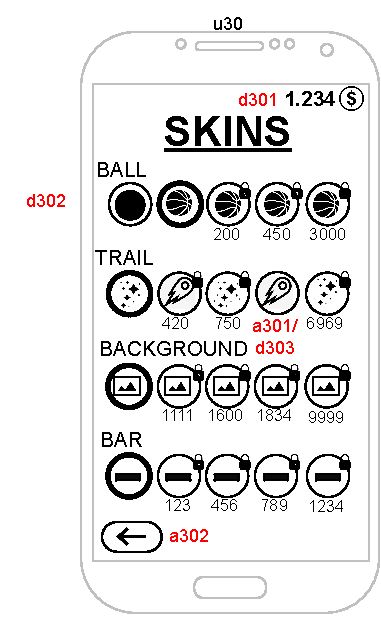
\includegraphics{diagramme/pdf/Mockup-u30.pdf}
\end{center}
    \caption{Dialog u30 - Skin Auswahl}
\end{wrapfigure}

Die Skin-Auswahl bietet dem \gls{spieler} fünf Skins, jeweils für den \gls{ball}, den Schweif, den Hintergrund und der Bar an.
Dem \gls{spieler} muss es möglich sein, durch einen Klick auf den Zurück-Pfeil wieder ins Hauptmenü zu gelangen.
\clearpage

\subsubsection{Dialog u31 - Skin Kauf}

\begin{wrapfigure}{l}{0.5\textwidth}
    \begin{center}
    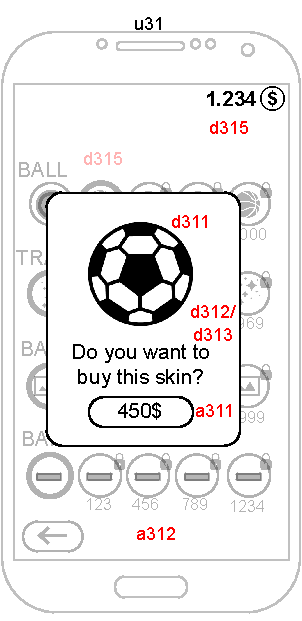
\includegraphics{diagramme/pdf/Mockup-u31.pdf}
\end{center}
    \caption{Dialog u31 - Skin Kauf}
\end{wrapfigure}

Kauft der \gls{spieler} einen Skin, so muss der Skin vergrößert angezeigt werden. Außerdem muss der Preis angezeigt werden.
\clearpage

\subsubsection{Dialog u40 - Credits}

\begin{wrapfigure}{l}{0.5\textwidth}
    \begin{center}
    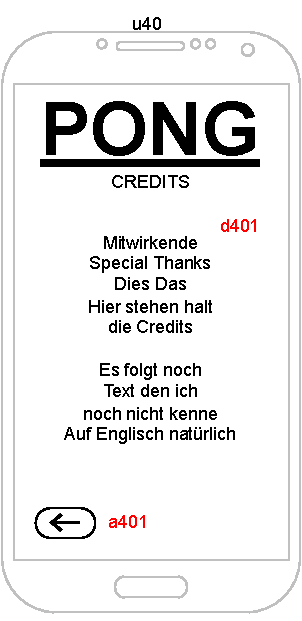
\includegraphics{diagramme/pdf/Mockup-u40.pdf}
    \caption{Dialog u40 - Credits}
    \end{center}
\end{wrapfigure}

Der \gls{spieler} muss die Möglichkeit haben in den Credits genauere Informationen zum Entwicklerteam, und zur App allgemein zu bekommen.
Durch einen Klick auf den zurück-Pfeil, muss der Nutzer wieder ins Hauptmenü gelangen.
\clearpage
    \clearpage

    \section{Produktdaten}\label{sec:produktdaten}
        \subsection{Systeme / Arbeitspakete}

\newcommand{\OPT}[1]{{\color{teal} #1}}


% use 2 variables for Category and System ref
\newcommand{\CAT}{F}
\newcommand{\SYS}{\ref*{sys:ui}}
\newcommand{\setCategory}[1]{ \gdef\CAT{#1} }
\newcommand{\setSystem}[1]{ \gdef\SYS{#1}\hspace*{-9px}\setcounter{rowcntr}{0} }

\newcounter{rowcntr}[table]                             % create a new counter
\AtBeginEnvironment{tabular}{\setcounter{rowcntr}{0}}   % Reset the rowcntr counter at each new tabular
\renewcommand{\therowcntr}{\CAT-\SYS-\arabic{rowcntr}}  % define the layout of the counter value

% \renewcommand{\therowcntr}{\thetable.\arabic{rowcntr}}
% % A new columntype to apply automatic stepping
% \newcolumntype{N}{>{\refstepcounter{rowcntr}\therowcntr}c}

% This function inserts the counter into a table row and creates a label at it's position
\newcommand{\REQ}[1]{
    \refstepcounter{rowcntr}
    \therowcntr
    \label{#1} 
}




Zur besseren Übersichtlichkeit und Verteilung kleinerer Aufgabenpakete wird die Applikation in folgende
Subsysteme unterteilt:

\begin{enumerate}
    \item \label{sys:gen} Generelles
    \item \label{sys:ui} User Interface \& Menüs
    \item \label{sys:ls} Life System
    \item \label{sys:cm} Classic-Mode
    \item \label{sys:inv} Invasion-Mode
    \item \label{sys:scs} Scoring System
    \item \label{sys:cur} Currency System
\end{enumerate}

\subsection{Requirements}

Requirements werden unterteilt in die folgenden Gruppen:

\begin{itemize}
    \item Functional: Funktionale Anforderungen
    \item Design: Rahmenanforderungen / Designbestimmungen
    \item Performance: Quantisierbare Leistungsanforderungen
    \item Operational: Nutzungsanforderungen und Umgebungseinschränkungen
\end{itemize}

Jedes Requirement besteht aus einer eindeutigen ID, die sich zusammensetzt aus:

\begin{itemize}
    \item Requirement Typ (F/D/P/O)
    \item Subsystem Nummer (1,2,3,4,5,6)
    \item Laufende Nummer
\end{itemize}

% Folgende Wörter werden wie folgt definiert

% \begin{itemize}
%     \item SEIN: beschreibt eine Funktion %lmao
%     \item MUSS: rechtlich bindend
%     \item SOLL: dringend empfohlen
%     \item WIRD: zukünftige Anforderung (eventuell Bestandteil eines späteren Releases)
% \end{itemize}


Die explizit mit \OPT{*} gekennzeichneten Requirements sind optionale Anforderungen, sogennante Nice-To-Haves.

\subsubsection{Functional Requirements}

\begin{xltabular}{\textwidth}{|l|X|r|r|}
    \hline
    \textbf{ID} & \textbf{Definition}   & \textbf{I}    & \textbf{QA}                                           \\
    \hline

    \setSystem{\ref*{sys:gen}}  % General

    \REQ{r:1}   & Das Spiel ist pausierbar.             &      &      \\ \hline
    \REQ{r:2}   & Das Spiel kann zu jeder Zeit beendet werden.             &      &      \\ \hline
    \REQ{r:8}   & Das Spiel ermöglicht die Steuerung des \glspl{balken} per Finger.             &      &     \\ \hline
    \REQ{r:8}   & Der \gls{balken} hat eine maximale Geschwindigkeit.        &           &         \\ \hline

    \setSystem{\ref*{sys:ui}}   % User Interface

    \REQ{r:3}   & \OPT{*} Der \gls{spieler} kann im \hyperref[fig:dia:mainMenu]{Hauptmenü} die Sprache wechseln.             &      &      \\ \hline
    \REQ{r:4}   & Der \gls{spieler} muss seinen Namen nach Ende des Spiels eingeben, sofern er einen neuen Highscore aufgestellt hat.        &      &      \\ \hline
    \REQ{r:5}   & \OPT{*} Bestimmte Aktionen im Spiel erzeugen Geräusche.             &      &      \\ \hline
    \REQ{r:6}   & Nach dem Drücken der Play-Taste werden die \hyperref[fig:dia:gameMode]{Spielmodus Einstellungen} angezeigt.             &      &      \\ \hline
    \REQ{r:7}   & In den \hyperref[fig:dia:gameMode]{Spielmodus Einstellungen} muss der Schwierigkeitsgrad gewählt werden.             &      &      \\ \hline
    \REQ{r:8}   & \OPT{*}In den \hyperref[fig:dia:gameMode]{Spielmodus Einstellungen} muss der Spielmodus gewählt werden.             &      &      \\ \hline
    
    \setSystem{\ref*{sys:ls}}   % Life System

    %\gls{leben}ssystem
    \REQ{r:9}   & Der \gls{spieler} hat eine Anzahl an \gls{leben}.             &      &      \\ \hline
    \REQ{r:10}  & Der \gls{spieler} muss ein \gls{leben} verlieren, wenn der \gls{ball} das \gls{spielfeld} verlässt. &      &      \\ \hline
    \REQ{r:11}  & Nach dem Verlust aller \gls{leben}, wird dem \gls{spieler} die Möglichkeit geboten, 1 \gls{leben} durch Ansehen eines Werbevideos wiederherzustellen.        &      &      \\ \hline

    \setSystem{\ref*{sys:cm}}   % Classic Mode
    
    \REQ{r:13}  & Das Spiel hat einen Hauptmodus - \gls{classicMode}.        &      &      \\ \hline
    \REQ{r:14}  & Der \gls{ball} prallt während des Spiels vom \gls{balken} ab.              &      &      \\ \hline
    \REQ{r:15}  & Am Anfang des Spiels ist der \gls{ball} mittig auf dem \gls{balken} positioniert.              &      &      \\ \hline
    \REQ{r:16}  & Beim einmaligen Tippen auf dem Bildschirm prallt der \gls{ball} vom \gls{balken} ab und das Spiel beginnt.              &      &      \\ \hline
    \REQ{r:17}  & Der \gls{ball} prallt von den Bildschirmrändern oben, rechts, links ab.              &      &      \\ \hline
    \REQ{r:18}  & Jedes Abprallen am \gls{balken} gibt einen \gls{point}.              &      &      \\ \hline
    \REQ{r:19}  & \OPT{*} Es soll ein Achievement-System geben. &      &   \\ \hline
    \REQ{r:20}  & \OPT{*} Im Spiel sollen unterschiedliche Spielboni auftreten.        &      &      \\ \hline
    \REQ{r:21}  & \OPT{*} Spielboni treten zufällig auf.              &      &      \\ \hline
    \REQ{r:22}  & \OPT{*} Spielboni dauern im \gls{classicMode} eine limitierte Zeit an, bevor sie wieder verschwinden.              &      &      \\ \hline
    \REQ{r:23}  & \OPT{*} Spielboni sind im \gls{invasionMode} persistent bis sie vom \gls{ball} getroffen und eingelöst werden.              &      &      \\ \hline
    \REQ{r:24}  & Der \gls{spieler} kann aus 3 Schwierigkeitsgraden wählen.        &      &      \\ \hline
    \REQ{r:25}  & \OPT{*} Einer der Spielboni ermöglicht es, ein \gls{leben} zurückzubekommen, falls ihre Anzahl kleiner 3 ist.            &      &      \\ \hline
    \REQ{r:26}  & \OPT{*} Einer der Spielboni macht den \gls{ball} für limitierte Zeit langsamer.            &      &      \\ \hline
    \REQ{r:27}  & \OPT{*} Einer der Spielboni macht den \gls{balken} für limitierte Zeit größer.            &      &      \\ \hline

    \setSystem{\ref*{sys:inv}}   % Invasion Mode

    \REQ{r:28}  & \OPT{*} Das Spiel hat einen Nebenmodus: \gls{invasionMode}.    &      &      \\ \hline
    \REQ{r:29}  & \OPT{*} Im \gls{invasionMode} kann der \gls{ball} \glspl{block} zerstören.    &      &      \\ \hline
    \REQ{r:30}  & \OPT{*} Nach einer festen Zeit erscheint eine neue Reihe von \glspl{block}.     &      &      \\ \hline
    \REQ{r:31}  & \OPT{*} Erreicht mindestens ein \gls{block} den unteren Rand des \gls{spielfeld}, verliert der \gls{spieler} 1 \gls{leben}.    &      &      \\ \hline
    \REQ{r:32}  & \OPT{*} Mit zunehmender Zeit erhöht sich die Anzahl der stärkeren \glspl{block}.    &      &      \\ \hline
    \REQ{r:33}  & \OPT{*} Ein \gls{block} mit Stärke N gibt N \gls{point} beim Zerstören.    &      &      \\ \hline
    \REQ{r:34}  & \OPT{*} Einer der Spielboni macht den \gls{ball} für limitierte Zeit stärker.            &      &      \\ \hline
    \REQ{r:35}  & \OPT{*} Einer der Spielboni ermöglicht das Zerstören der Reihe, in der er liegt.            &      &      \\ \hline
    \REQ{r:36}  & \OPT{*} Einer der Spielboni ermöglicht das Zerstören aller umliegenden \glspl{block}.            &      &      \\ \hline

    \setSystem{\ref*{sys:scs}}   % Scoring System
    
    \REQ{r:37}  & Am Ende des Spiels erscheint eine \hyperref[fig:dia:gameOver]{Übersicht}. &      &      \\ \hline
    \REQ{r:38}  & In der \hyperref[fig:dia:gameOver]{Übersicht} werden die erreichten \glspl{point}, verdienten \glspl{coin} und Spielzeit angezeigt. &      &      \\ \hline
    \REQ{r:39}  & Falls bei Spielende ein Score höher als der 10. Score der \hyperref[fig:dia:top10]{Top10-Liste} erreicht, wird die \hyperref[fig:dia:top10]{Liste} entsprechend aktualisiert. &      &      \\ \hline
    \REQ{r:40}  & Falls die \hyperref[fig:dia:top10]{Liste} aktualisiert wurde, wird der \gls{spieler} nach dem Spiel aufgefordert, im entsprechenden \hyperref[fig:dia:fig:dia:highscore]{Menü} seinen Namen einzugeben.             &      &      \\ \hline
    \REQ{r:41}  & \OPT{*}Es gibt eine Top10 Highscore Tabelle pro Spielmodus.            &      &      \\ \hline
    \REQ{r:42}  & Pro Schwierigkeitsstufe gibt es einen unterschiedlichen \glspl{point}-Multiplier.             &      &      \\ \hline

    \setSystem{\ref*{sys:cur}}   % Currency System
    
    \REQ{r:43}  & Für alle 10 \glspl{point} verdient der \gls{spieler} einen \gls{coin}. &      &      \\ \hline %Kunde will das so haben
    \REQ{r:44}  & \glspl{coin} schalten \glspl{skin} für den \gls{ball} frei.           &      &      \\ \hline
    \REQ{r:45}  & \glspl{coin} schalten \glspl{skin} für den \gls{balken} frei.           &      &      \\ \hline % entweder \glspl{skin} oder PowerUp Overlay - Kunde überlegt noch, Stand: 28.10.2022
    \REQ{r:46}  & \glspl{coin} schalten \glspl{skin} für den Hintergrund frei.           &      &      \\ \hline
    \REQ{r:47}  & \glspl{coin} schalten \glspl{skin} für den \gls{tail} des \glspl{ball} frei.           &      &      \\ \hline

    \caption{Funktionale Anforderungen}\label{tab:functional-requirements}
\end{xltabular}

\clearpage

\subsubsection{Design Requirements}
\renewcommand{\CAT}{D}
\begin{xltabular}{\textwidth}{|l|X|r|r|}
    \hline
    \textbf{ID} & \textbf{Definition}   & \textbf{I}    & \textbf{QA}                                           \\
    \hline

    \setSystem{\ref*{sys:gen}}  % General

    \REQ{r:48}  & Die gesammte Applikation läuft als Singleplayer.             &      &     \\ \hline
    \REQ{r:49}  & Die gesammte Applikation läuft offline.             &      &      \\ \hline
    \REQ{r:50}  & Der Name des Spiels ist Pong.             &      &     \\ \hline
    \REQ{r:51}  & Die Ausrichtung des Spiels ist hochkant.             &      &     \\ \hline
    \REQ{r:52}  & Das Haupttheme des Spiels ist dunkel mit hellen Akzenten / Space-Theme.      &      &     \\ \hline
    \REQ{r:53}  & Der \gls{ball} besitzt einen \gls{tail}.             &      &      \\ \hline
    \REQ{r:73}  & Die Wiederherstellung eines \glspl{leben} durch Werbung (siehe \ref{r:11}) ist nur einmalig möglich. &   &  \\ \hline

    \setSystem{\ref*{sys:ui}}  % User Interface

    \REQ{r:54}  & Die im Spiel verwendete Sprache ist Englisch.             &      &      \\ \hline
    \REQ{r:55}  & Die \glspl{leben}-Anzeige des Spiels wird Herzen angezeigt.             &     &      \\ \hline
    \REQ{r:56}  & Die Herzen der \glspl{leben}-Anzeige sind rot.             &     &      \\ \hline
    \REQ{r:57}  & Buttons haben eine abgerundete Form / border-radius.             &      &      \\ \hline
    \REQ{r:58}  & Alle Menüs haben denselben Hintergrund wie im Spiel, nämlich der aktuell gewählte.             &     &      \\ \hline
    \REQ{r:59}  & Die wählbaren Hintergrüned sind dunkel, aber nicht einfarbig.             &     &      \\ \hline
    \REQ{r:60}  & Die Schriftfarbe muss einen hohen Kontrast zum Hintergrund haben. &  &  \\ \hline 
    %Startbildschirm
    \REQ{r:61}  & Am Anfang des Spiels wird ein \hyperref[fig:dia:mainMenu]{Startbildschirm} angezeigt.             &      &      \\ \hline
    \REQ{r:62}  & Auf dem \hyperref[fig:dia:mainMenu]{Startbildschirm} wird die Taste "Play" angezeigt.             &      &      \\ \hline
    \REQ{r:63}  & Auf dem \hyperref[fig:dia:mainMenu]{Startbildschirm} wird die Taste "Top 10" angezeigt.             &      &      \\ \hline
    \REQ{r:64}  & Auf dem \hyperref[fig:dia:mainMenu]{Startbildschirm} wird die Taste "Credits" angezeigt.             &      &      \\ \hline
    \REQ{r:65}  & Auf dem \hyperref[fig:dia:mainMenu]{Startbildschirm} wird die Taste "Skins" angezeigt.             &      &      \\ \hline
    \REQ{r:66}  & Auf dem \hyperref[fig:dia:mainMenu]{Startbildschirm} wird die Taste mit der aktuellen Sprache angezeigt.             &      &      \\ \hline
    %Spielbildschirm
    \REQ{r:67}  & Im \hyperref[fig:dia:gameMode]{Spielbildschirm} wird zuerst der Spielmodus und darunter der Schweirigkeitsgrad angezeigt.             &      &      \\ \hline
    \REQ{r:68}  & Im Spiel (\hyperref[fig:dia:fig:dia:classic]{Classic}/\hyperref[fig:dia:invasion]{Invasion}) wird eine Headerleiste angezeigt.             &     &      \\ \hline
    \REQ{r:69}  & In der Headerleiste werden links die \gls{leben} angezeigt.             &      &      \\ \hline
    \REQ{r:70}  & In der Headerleiste werden in der Mitte die aktuellen \glspl{point} angezeigt.             &      &      \\ \hline 
    \REQ{r:71}  & Der Punktstand (\glspl{point}) wird ohne führende Nullen angezeigt.             &      &      \\ \hline
    \REQ{r:72}  & In der Headerleiste wird rechts die Pause-Taste angezeigt.             &      &      \\ \hline
    %Endbildschirm Summary
    
    \setSystem{\ref*{sys:cm}}   % Classic Mode

    \REQ{r:81}  & Der Abprall des \glspl{ball} an den Wänden hängt vom Eintrittswinkel ab.             &      &      \\ \hline
    \REQ{r:82}  & Der Abprall des \glspl{ball} am \gls{balken} hängt vom Eintrittswinkel und Auftreffpunkt ab.             &      &      \\ \hline
    \REQ{r:83}  & \OPT{*} Die Spielboni sind visuell dargestellt.        &      &      \\ \hline
    %Schwierigkeitsgrad
    \REQ{r:84}  & Auf Schwierigkeitsgrad "Easy" bleibt der \gls{ball} auf normale Geschwindigkeit.              &      &      \\ \hline
    \REQ{r:85}  & Auf Schwierigkeitsgrad "Easy" ist der \gls{balken} größer.              &      &      \\ \hline
    \REQ{r:86}  & Auf Schwierigkeitsgrad "Medium" ist der \gls{balken} mittelgroß.            &      &      \\ \hline
    \REQ{r:87}  & Auf Schwierigkeitsgrad "Medium" wird der \gls{ball} bis zu einem von den Entwicklern bestimmten Hochpunkt schneller.             &      &      \\ \hline
    \REQ{r:88}  & Auf Schwierigkeitsgrad "Hard" steigt die Geschwindigkeit des \glspl{ball} mit einer schnelleren Rate.             &      &      \\ \hline
    \REQ{r:89}  & Auf Schweirigkeitsgrad "Hard" ist die maximale Geschwindigkeit des \glspl{ball} größer als auf "Medium".             &      &      \\ \hline
    \REQ{r:90}  & Auf Schwierigkeitsgrad "Hard" ist der \gls{balken} klein.             &      &      \\ \hline

    \setSystem{\ref*{sys:inv}}   % Invasion Mode

    \REQ{r:96}  & \OPT{*} Im \gls{invasionMode} ist die \gls{ball}-Größe ca. 80\% der \gls{block}-Größe.            &      &      \\ \hline
    \REQ{r:97}  & \OPT{*} Jeder \gls{block} besitzt eine individuelle Stärke/HP.    &      &      \\ \hline
    \REQ{r:98}  & \OPT{*} Die Stärke (vgl. \ref{r:97}) der liegt zwischen 1 und 6, inklusive.    &      &      \\ \hline
    \REQ{r:99}  & \OPT{*} Die Farbe jedes \glspl{block} ist je nach Stärke (vgl. \ref{r:97}) unterschiedlich.    &      &      \\ \hline
    \REQ{r:100} & \OPT{*} Pro Reihe gibt es 6 \glspl{block}.    &      &      \\ \hline

    \setSystem{\ref*{sys:scs}}   % Scoring System

    \REQ{r:75}  & Solange der \gls{point}-Score wegen \glspl{powerup} verdoppelt wird, steht unter dem aktuellen Punktstand "2x".              &      &      \\ \hline
    \REQ{r:77}  & Jedes Element aus der \hyperref[fig:dia:top10]{Top10-Liste} besteht aus Position, Namen, Punktstand und Spielzeit.         &      &      \\ \hline
    \REQ{r:78}  & In der \hyperref[fig:dia:top10]{Top10-Liste} wird die Schwierigkeitsstufe durch eine entsprechende Farbe der Zeile gezeigt. &      &     \\ \hline
    \REQ{r:105} &  \gls{coin}-Stand wird im \hyperref[fig:dia:mainMenu]{Hauptmenü} \& \hyperref[fig:dia:skins]{Shop} angezeigt.            &      &      \\ \hline
    \REQ{r:101} &  Der gleiche Name kann mehrmals in der \hyperref[fig:dia:top10]{Top10-Liste} auftauchen.             &      &      \\ \hline
    \REQ{r:102} &  Der erreichte \gls{point}-Score wird am Ende jedes Spiels in der \hyperref[fig:dia:gameOver]{Übersicht} angezeigt.            &      &      \\ \hline
    \REQ{r:103} &  Die erreichte \gls{coin} Anzahl wird am Ende jedes Spiels in der \hyperref[fig:dia:gameOver]{Übersicht} angezeigt.            &      &      \\ \hline

    \setSystem{\ref*{sys:cur}}   % Currency System

    \REQ{r:104} &  Die Währung für den Shop heißt "\glspl{coin}".         &      &      \\ \hline
    \REQ{r:79}  & Es gibt einen Default-\gls{skin}.           &      &      \\ \hline
    \REQ{r:80}  & \glspl{skin} sind in verschiedenen Kategorien je nach Elementtyp(\gls{ball}, \gls{balken}, \gls{tail}, Hintergrund) unterteilt.           &      &      \\ \hline
    \REQ{r:74}  & Pro Kategorie gibt es mindestens 5 freischaltbare \glspl{skin}.           &      &      \\ \hline
    \REQ{r:106} & Die \glspl{skin} werden pro Kategorie sukzessiv teurer.           &      &      \\ \hline
    \REQ{r:91}  &  Der 1. \gls{skin} wird nach etwa 2 Spielen freigeschaltet.            &      &      \\ \hline %bleibt wegen Balancing, so der Kunde
    \REQ{r:92}  &  Der 2. \gls{skin} wird nach etwa 5 Spielen freigeschaltet.            &      &      \\ \hline
    \REQ{r:93}  &  Der 3. \gls{skin} wird nach etwa 10 Spielen freigeschaltet.            &      &      \\ \hline
    \REQ{r:94}  &  Der 4. \gls{skin} wird nach etwa 20 Spielen freigeschaltet.            &      &      \\ \hline
    \REQ{r:95}  &  Der 5. \gls{skin} wird nach etwa 30 Spielen freigeschaltet.            &      &      \\ \hline
    
    \caption{Design Anforderungen}\label{tab:design-requirements}
\end{xltabular}

\clearpage

\subsubsection{Performance Requirements}
\renewcommand{\CAT}{P}
\begin{xltabular}{\textwidth}{|l|X|r|r|}
    \hline
    \textbf{ID} & \textbf{Definition}   & \textbf{I}    & \textbf{QA}                                           \\
    \hline

    \setSystem{\ref*{sys:gen}}   % Life System

    \REQ{r:112} & \gls{ladezeiten} müssen unter 5 Sekunden liegen.        &     &      \\ \hline

    \setSystem{\ref*{sys:ls}}   % Life System

    \REQ{r:107} & Das Spiel startet mit 3 \gls{leben}.             &     &      \\ \hline

    \setSystem{\ref*{sys:cm}}   % Classic Mode

    \REQ{r:108} & Eine Spielrunde im Schweirigkeitsgrad "Medium" soll im Schnitt etwa 5 Minuten dauern.             &      &      \\ \hline
    \REQ{r:109} & Die verlangsamte Geschwindigkeit des \glspl{ball} beträgt etwa 70\% der normalen. &   &    \\ \hline

    \caption{Performance Anforderungen}\label{tab:performance-requirements}
\end{xltabular}

\subsubsection{Operational Requirements}
\renewcommand{\CAT}{O}
\begin{xltabular}{\textwidth}{|l|X|r|r|}
    \hline
    \textbf{ID} & \textbf{Definition}   & \textbf{I}    & \textbf{QA}                                           \\
    \hline

    \setSystem{\ref*{sys:gen}}  % General

    \REQ{r:110} & Das Spiel ist nur unter Android lauffähig.               &      &      \\ \hline
    
    \setSystem{\ref*{sys:ui}}   % User Interface

    \REQ{r:111} & Das Spiel muss entsprechend der Bildschirmmaße skaliert werden.             &      &      \\ \hline
    
    \caption{Operationale Anforderungen}\label{tab:operational-requirements}
\end{xltabular}

    \clearpage

    \section{Produktleistung, Performance}\label{sec:performance}
        Die App \gls{muss} alle Funktionen des Spiels in angemessener Zeit durchführen. 
Während des Spiels \gls{muss} es die Möglichkeit zur Pausierung geben.
Schließen der App, während man im Spiel ist, \gls{muss} das Spiel pausieren.
Die Framerate ist von der Hardware abhängig und kann somit nicht garantiert werden.
Nach einem Neustart der App müssen alle Highscores, Skins und Einstellungen gespeichert bleiben. 
    \clearpage

    \section{Qualitätsanforderungen}\label{sec:quality}
        \subsection{Bedienbarkeit \& Zuverlässigkeit \& Effizienz}\label{subsec:bedienbarkeit}
        Das Spiel Pong \gls{muss} auf allen Mobilgeräten mit Android Betriebssystem fehlerfrei laufen und bedienbar sein. Dabei gilt, dass das Endgerät mindestens mit Android 10 und darüber laufen \gls{muss}, um versionsbedingte Fehler zu vermeiden. Des Weiteren \gls{muss} sichergestellt werden, dass keine Fehler auftreten, die vom Programmcode des Spiels ausgehen.  

        \subsection{Anforderungen an die Änderbarkeit}
        Bei der Entwicklung der Software für das Spiel Pong \gls{muss} sich an gängige Konventionen gehalten werden, um zu gewährleisten, dass das Ändern oder Hinzufügen von Programmcode möglichst einfach stattfinden kann. 

        \subsection{Anforderungen an die Darstellung}
        Das Spiel wird im Hochkant Format ausgeführt und \gls{muss} abhängig von der Bildschirmgröße passend skaliert sein. 
    \clearpage

    \section{Tabellarische Requirements}\label{sec:requirements}
        \subsection{Systeme / Arbeitspakete}

\newcommand{\OPT}[1]{{\color{teal} #1}}


% use 2 variables for Category and System ref
\newcommand{\CAT}{F}
\newcommand{\SYS}{\ref*{sys:ui}}
\newcommand{\setCategory}[1]{ \gdef\CAT{#1} }
\newcommand{\setSystem}[1]{ \gdef\SYS{#1}\hspace*{-9px}\setcounter{rowcntr}{0} }

\newcounter{rowcntr}[table]                             % create a new counter
\AtBeginEnvironment{tabular}{\setcounter{rowcntr}{0}}   % Reset the rowcntr counter at each new tabular
\renewcommand{\therowcntr}{\CAT-\SYS-\arabic{rowcntr}}  % define the layout of the counter value

% \renewcommand{\therowcntr}{\thetable.\arabic{rowcntr}}
% % A new columntype to apply automatic stepping
% \newcolumntype{N}{>{\refstepcounter{rowcntr}\therowcntr}c}

% This function inserts the counter into a table row and creates a label at it's position
\newcommand{\REQ}[1]{
    \refstepcounter{rowcntr}
    \therowcntr
    \label{#1} 
}




Zur besseren Übersichtlichkeit und Verteilung kleinerer Aufgabenpakete wird die Applikation in folgende
Subsysteme unterteilt:

\begin{enumerate}
    \item \label{sys:gen} Generelles
    \item \label{sys:ui} User Interface \& Menüs
    \item \label{sys:ls} Life System
    \item \label{sys:cm} Classic-Mode
    \item \label{sys:inv} Invasion-Mode
    \item \label{sys:scs} Scoring System
    \item \label{sys:cur} Currency System
\end{enumerate}

\subsection{Requirements}

Requirements werden unterteilt in die folgenden Gruppen:

\begin{itemize}
    \item Functional: Funktionale Anforderungen
    \item Design: Rahmenanforderungen / Designbestimmungen
    \item Performance: Quantisierbare Leistungsanforderungen
    \item Operational: Nutzungsanforderungen und Umgebungseinschränkungen
\end{itemize}

Jedes Requirement besteht aus einer eindeutigen ID, die sich zusammensetzt aus:

\begin{itemize}
    \item Requirement Typ (F/D/P/O)
    \item Subsystem Nummer (1,2,3,4,5,6)
    \item Laufende Nummer
\end{itemize}

% Folgende Wörter werden wie folgt definiert

% \begin{itemize}
%     \item SEIN: beschreibt eine Funktion %lmao
%     \item MUSS: rechtlich bindend
%     \item SOLL: dringend empfohlen
%     \item WIRD: zukünftige Anforderung (eventuell Bestandteil eines späteren Releases)
% \end{itemize}


Die explizit mit \OPT{*} gekennzeichneten Requirements sind optionale Anforderungen, sogennante Nice-To-Haves.

\subsubsection{Functional Requirements}

\begin{xltabular}{\textwidth}{|l|X|r|r|}
    \hline
    \textbf{ID} & \textbf{Definition}   & \textbf{I}    & \textbf{QA}                                           \\
    \hline

    \setSystem{\ref*{sys:gen}}  % General

    \REQ{r:1}   & Das Spiel ist pausierbar.             &      &      \\ \hline
    \REQ{r:2}   & Das Spiel kann zu jeder Zeit beendet werden.             &      &      \\ \hline
    \REQ{r:8}   & Das Spiel ermöglicht die Steuerung des \glspl{balken} per Finger.             &      &     \\ \hline
    \REQ{r:8}   & Der \gls{balken} hat eine maximale Geschwindigkeit.        &           &         \\ \hline

    \setSystem{\ref*{sys:ui}}   % User Interface

    \REQ{r:3}   & \OPT{*} Der \gls{spieler} kann im \hyperref[fig:dia:mainMenu]{Hauptmenü} die Sprache wechseln.             &      &      \\ \hline
    \REQ{r:4}   & Der \gls{spieler} muss seinen Namen nach Ende des Spiels eingeben, sofern er einen neuen Highscore aufgestellt hat.        &      &      \\ \hline
    \REQ{r:5}   & \OPT{*} Bestimmte Aktionen im Spiel erzeugen Geräusche.             &      &      \\ \hline
    \REQ{r:6}   & Nach dem Drücken der Play-Taste werden die \hyperref[fig:dia:gameMode]{Spielmodus Einstellungen} angezeigt.             &      &      \\ \hline
    \REQ{r:7}   & In den \hyperref[fig:dia:gameMode]{Spielmodus Einstellungen} muss der Schwierigkeitsgrad gewählt werden.             &      &      \\ \hline
    \REQ{r:8}   & \OPT{*}In den \hyperref[fig:dia:gameMode]{Spielmodus Einstellungen} muss der Spielmodus gewählt werden.             &      &      \\ \hline
    
    \setSystem{\ref*{sys:ls}}   % Life System

    %\gls{leben}ssystem
    \REQ{r:9}   & Der \gls{spieler} hat eine Anzahl an \gls{leben}.             &      &      \\ \hline
    \REQ{r:10}  & Der \gls{spieler} muss ein \gls{leben} verlieren, wenn der \gls{ball} das \gls{spielfeld} verlässt. &      &      \\ \hline
    \REQ{r:11}  & Nach dem Verlust aller \gls{leben}, wird dem \gls{spieler} die Möglichkeit geboten, 1 \gls{leben} durch Ansehen eines Werbevideos wiederherzustellen.        &      &      \\ \hline

    \setSystem{\ref*{sys:cm}}   % Classic Mode
    
    \REQ{r:13}  & Das Spiel hat einen Hauptmodus - \gls{classicMode}.        &      &      \\ \hline
    \REQ{r:14}  & Der \gls{ball} prallt während des Spiels vom \gls{balken} ab.              &      &      \\ \hline
    \REQ{r:15}  & Am Anfang des Spiels ist der \gls{ball} mittig auf dem \gls{balken} positioniert.              &      &      \\ \hline
    \REQ{r:16}  & Beim einmaligen Tippen auf dem Bildschirm prallt der \gls{ball} vom \gls{balken} ab und das Spiel beginnt.              &      &      \\ \hline
    \REQ{r:17}  & Der \gls{ball} prallt von den Bildschirmrändern oben, rechts, links ab.              &      &      \\ \hline
    \REQ{r:18}  & Jedes Abprallen am \gls{balken} gibt einen \gls{point}.              &      &      \\ \hline
    \REQ{r:19}  & \OPT{*} Es soll ein Achievement-System geben. &      &   \\ \hline
    \REQ{r:20}  & \OPT{*} Im Spiel sollen unterschiedliche Spielboni auftreten.        &      &      \\ \hline
    \REQ{r:21}  & \OPT{*} Spielboni treten zufällig auf.              &      &      \\ \hline
    \REQ{r:22}  & \OPT{*} Spielboni dauern im \gls{classicMode} eine limitierte Zeit an, bevor sie wieder verschwinden.              &      &      \\ \hline
    \REQ{r:23}  & \OPT{*} Spielboni sind im \gls{invasionMode} persistent bis sie vom \gls{ball} getroffen und eingelöst werden.              &      &      \\ \hline
    \REQ{r:24}  & Der \gls{spieler} kann aus 3 Schwierigkeitsgraden wählen.        &      &      \\ \hline
    \REQ{r:25}  & \OPT{*} Einer der Spielboni ermöglicht es, ein \gls{leben} zurückzubekommen, falls ihre Anzahl kleiner 3 ist.            &      &      \\ \hline
    \REQ{r:26}  & \OPT{*} Einer der Spielboni macht den \gls{ball} für limitierte Zeit langsamer.            &      &      \\ \hline
    \REQ{r:27}  & \OPT{*} Einer der Spielboni macht den \gls{balken} für limitierte Zeit größer.            &      &      \\ \hline

    \setSystem{\ref*{sys:inv}}   % Invasion Mode

    \REQ{r:28}  & \OPT{*} Das Spiel hat einen Nebenmodus: \gls{invasionMode}.    &      &      \\ \hline
    \REQ{r:29}  & \OPT{*} Im \gls{invasionMode} kann der \gls{ball} \glspl{block} zerstören.    &      &      \\ \hline
    \REQ{r:30}  & \OPT{*} Nach einer festen Zeit erscheint eine neue Reihe von \glspl{block}.     &      &      \\ \hline
    \REQ{r:31}  & \OPT{*} Erreicht mindestens ein \gls{block} den unteren Rand des \gls{spielfeld}, verliert der \gls{spieler} 1 \gls{leben}.    &      &      \\ \hline
    \REQ{r:32}  & \OPT{*} Mit zunehmender Zeit erhöht sich die Anzahl der stärkeren \glspl{block}.    &      &      \\ \hline
    \REQ{r:33}  & \OPT{*} Ein \gls{block} mit Stärke N gibt N \gls{point} beim Zerstören.    &      &      \\ \hline
    \REQ{r:34}  & \OPT{*} Einer der Spielboni macht den \gls{ball} für limitierte Zeit stärker.            &      &      \\ \hline
    \REQ{r:35}  & \OPT{*} Einer der Spielboni ermöglicht das Zerstören der Reihe, in der er liegt.            &      &      \\ \hline
    \REQ{r:36}  & \OPT{*} Einer der Spielboni ermöglicht das Zerstören aller umliegenden \glspl{block}.            &      &      \\ \hline

    \setSystem{\ref*{sys:scs}}   % Scoring System
    
    \REQ{r:37}  & Am Ende des Spiels erscheint eine \hyperref[fig:dia:gameOver]{Übersicht}. &      &      \\ \hline
    \REQ{r:38}  & In der \hyperref[fig:dia:gameOver]{Übersicht} werden die erreichten \glspl{point}, verdienten \glspl{coin} und Spielzeit angezeigt. &      &      \\ \hline
    \REQ{r:39}  & Falls bei Spielende ein Score höher als der 10. Score der \hyperref[fig:dia:top10]{Top10-Liste} erreicht, wird die \hyperref[fig:dia:top10]{Liste} entsprechend aktualisiert. &      &      \\ \hline
    \REQ{r:40}  & Falls die \hyperref[fig:dia:top10]{Liste} aktualisiert wurde, wird der \gls{spieler} nach dem Spiel aufgefordert, im entsprechenden \hyperref[fig:dia:fig:dia:highscore]{Menü} seinen Namen einzugeben.             &      &      \\ \hline
    \REQ{r:41}  & \OPT{*}Es gibt eine Top10 Highscore Tabelle pro Spielmodus.            &      &      \\ \hline
    \REQ{r:42}  & Pro Schwierigkeitsstufe gibt es einen unterschiedlichen \glspl{point}-Multiplier.             &      &      \\ \hline

    \setSystem{\ref*{sys:cur}}   % Currency System
    
    \REQ{r:43}  & Für alle 10 \glspl{point} verdient der \gls{spieler} einen \gls{coin}. &      &      \\ \hline %Kunde will das so haben
    \REQ{r:44}  & \glspl{coin} schalten \glspl{skin} für den \gls{ball} frei.           &      &      \\ \hline
    \REQ{r:45}  & \glspl{coin} schalten \glspl{skin} für den \gls{balken} frei.           &      &      \\ \hline % entweder \glspl{skin} oder PowerUp Overlay - Kunde überlegt noch, Stand: 28.10.2022
    \REQ{r:46}  & \glspl{coin} schalten \glspl{skin} für den Hintergrund frei.           &      &      \\ \hline
    \REQ{r:47}  & \glspl{coin} schalten \glspl{skin} für den \gls{tail} des \glspl{ball} frei.           &      &      \\ \hline

    \caption{Funktionale Anforderungen}\label{tab:functional-requirements}
\end{xltabular}

\clearpage

\subsubsection{Design Requirements}
\renewcommand{\CAT}{D}
\begin{xltabular}{\textwidth}{|l|X|r|r|}
    \hline
    \textbf{ID} & \textbf{Definition}   & \textbf{I}    & \textbf{QA}                                           \\
    \hline

    \setSystem{\ref*{sys:gen}}  % General

    \REQ{r:48}  & Die gesammte Applikation läuft als Singleplayer.             &      &     \\ \hline
    \REQ{r:49}  & Die gesammte Applikation läuft offline.             &      &      \\ \hline
    \REQ{r:50}  & Der Name des Spiels ist Pong.             &      &     \\ \hline
    \REQ{r:51}  & Die Ausrichtung des Spiels ist hochkant.             &      &     \\ \hline
    \REQ{r:52}  & Das Haupttheme des Spiels ist dunkel mit hellen Akzenten / Space-Theme.      &      &     \\ \hline
    \REQ{r:53}  & Der \gls{ball} besitzt einen \gls{tail}.             &      &      \\ \hline
    \REQ{r:73}  & Die Wiederherstellung eines \glspl{leben} durch Werbung (siehe \ref{r:11}) ist nur einmalig möglich. &   &  \\ \hline

    \setSystem{\ref*{sys:ui}}  % User Interface

    \REQ{r:54}  & Die im Spiel verwendete Sprache ist Englisch.             &      &      \\ \hline
    \REQ{r:55}  & Die \glspl{leben}-Anzeige des Spiels wird Herzen angezeigt.             &     &      \\ \hline
    \REQ{r:56}  & Die Herzen der \glspl{leben}-Anzeige sind rot.             &     &      \\ \hline
    \REQ{r:57}  & Buttons haben eine abgerundete Form / border-radius.             &      &      \\ \hline
    \REQ{r:58}  & Alle Menüs haben denselben Hintergrund wie im Spiel, nämlich der aktuell gewählte.             &     &      \\ \hline
    \REQ{r:59}  & Die wählbaren Hintergrüned sind dunkel, aber nicht einfarbig.             &     &      \\ \hline
    \REQ{r:60}  & Die Schriftfarbe muss einen hohen Kontrast zum Hintergrund haben. &  &  \\ \hline 
    %Startbildschirm
    \REQ{r:61}  & Am Anfang des Spiels wird ein \hyperref[fig:dia:mainMenu]{Startbildschirm} angezeigt.             &      &      \\ \hline
    \REQ{r:62}  & Auf dem \hyperref[fig:dia:mainMenu]{Startbildschirm} wird die Taste "Play" angezeigt.             &      &      \\ \hline
    \REQ{r:63}  & Auf dem \hyperref[fig:dia:mainMenu]{Startbildschirm} wird die Taste "Top 10" angezeigt.             &      &      \\ \hline
    \REQ{r:64}  & Auf dem \hyperref[fig:dia:mainMenu]{Startbildschirm} wird die Taste "Credits" angezeigt.             &      &      \\ \hline
    \REQ{r:65}  & Auf dem \hyperref[fig:dia:mainMenu]{Startbildschirm} wird die Taste "Skins" angezeigt.             &      &      \\ \hline
    \REQ{r:66}  & Auf dem \hyperref[fig:dia:mainMenu]{Startbildschirm} wird die Taste mit der aktuellen Sprache angezeigt.             &      &      \\ \hline
    %Spielbildschirm
    \REQ{r:67}  & Im \hyperref[fig:dia:gameMode]{Spielbildschirm} wird zuerst der Spielmodus und darunter der Schweirigkeitsgrad angezeigt.             &      &      \\ \hline
    \REQ{r:68}  & Im Spiel (\hyperref[fig:dia:fig:dia:classic]{Classic}/\hyperref[fig:dia:invasion]{Invasion}) wird eine Headerleiste angezeigt.             &     &      \\ \hline
    \REQ{r:69}  & In der Headerleiste werden links die \gls{leben} angezeigt.             &      &      \\ \hline
    \REQ{r:70}  & In der Headerleiste werden in der Mitte die aktuellen \glspl{point} angezeigt.             &      &      \\ \hline 
    \REQ{r:71}  & Der Punktstand (\glspl{point}) wird ohne führende Nullen angezeigt.             &      &      \\ \hline
    \REQ{r:72}  & In der Headerleiste wird rechts die Pause-Taste angezeigt.             &      &      \\ \hline
    %Endbildschirm Summary
    
    \setSystem{\ref*{sys:cm}}   % Classic Mode

    \REQ{r:81}  & Der Abprall des \glspl{ball} an den Wänden hängt vom Eintrittswinkel ab.             &      &      \\ \hline
    \REQ{r:82}  & Der Abprall des \glspl{ball} am \gls{balken} hängt vom Eintrittswinkel und Auftreffpunkt ab.             &      &      \\ \hline
    \REQ{r:83}  & \OPT{*} Die Spielboni sind visuell dargestellt.        &      &      \\ \hline
    %Schwierigkeitsgrad
    \REQ{r:84}  & Auf Schwierigkeitsgrad "Easy" bleibt der \gls{ball} auf normale Geschwindigkeit.              &      &      \\ \hline
    \REQ{r:85}  & Auf Schwierigkeitsgrad "Easy" ist der \gls{balken} größer.              &      &      \\ \hline
    \REQ{r:86}  & Auf Schwierigkeitsgrad "Medium" ist der \gls{balken} mittelgroß.            &      &      \\ \hline
    \REQ{r:87}  & Auf Schwierigkeitsgrad "Medium" wird der \gls{ball} bis zu einem von den Entwicklern bestimmten Hochpunkt schneller.             &      &      \\ \hline
    \REQ{r:88}  & Auf Schwierigkeitsgrad "Hard" steigt die Geschwindigkeit des \glspl{ball} mit einer schnelleren Rate.             &      &      \\ \hline
    \REQ{r:89}  & Auf Schweirigkeitsgrad "Hard" ist die maximale Geschwindigkeit des \glspl{ball} größer als auf "Medium".             &      &      \\ \hline
    \REQ{r:90}  & Auf Schwierigkeitsgrad "Hard" ist der \gls{balken} klein.             &      &      \\ \hline

    \setSystem{\ref*{sys:inv}}   % Invasion Mode

    \REQ{r:96}  & \OPT{*} Im \gls{invasionMode} ist die \gls{ball}-Größe ca. 80\% der \gls{block}-Größe.            &      &      \\ \hline
    \REQ{r:97}  & \OPT{*} Jeder \gls{block} besitzt eine individuelle Stärke/HP.    &      &      \\ \hline
    \REQ{r:98}  & \OPT{*} Die Stärke (vgl. \ref{r:97}) der liegt zwischen 1 und 6, inklusive.    &      &      \\ \hline
    \REQ{r:99}  & \OPT{*} Die Farbe jedes \glspl{block} ist je nach Stärke (vgl. \ref{r:97}) unterschiedlich.    &      &      \\ \hline
    \REQ{r:100} & \OPT{*} Pro Reihe gibt es 6 \glspl{block}.    &      &      \\ \hline

    \setSystem{\ref*{sys:scs}}   % Scoring System

    \REQ{r:75}  & Solange der \gls{point}-Score wegen \glspl{powerup} verdoppelt wird, steht unter dem aktuellen Punktstand "2x".              &      &      \\ \hline
    \REQ{r:77}  & Jedes Element aus der \hyperref[fig:dia:top10]{Top10-Liste} besteht aus Position, Namen, Punktstand und Spielzeit.         &      &      \\ \hline
    \REQ{r:78}  & In der \hyperref[fig:dia:top10]{Top10-Liste} wird die Schwierigkeitsstufe durch eine entsprechende Farbe der Zeile gezeigt. &      &     \\ \hline
    \REQ{r:105} &  \gls{coin}-Stand wird im \hyperref[fig:dia:mainMenu]{Hauptmenü} \& \hyperref[fig:dia:skins]{Shop} angezeigt.            &      &      \\ \hline
    \REQ{r:101} &  Der gleiche Name kann mehrmals in der \hyperref[fig:dia:top10]{Top10-Liste} auftauchen.             &      &      \\ \hline
    \REQ{r:102} &  Der erreichte \gls{point}-Score wird am Ende jedes Spiels in der \hyperref[fig:dia:gameOver]{Übersicht} angezeigt.            &      &      \\ \hline
    \REQ{r:103} &  Die erreichte \gls{coin} Anzahl wird am Ende jedes Spiels in der \hyperref[fig:dia:gameOver]{Übersicht} angezeigt.            &      &      \\ \hline

    \setSystem{\ref*{sys:cur}}   % Currency System

    \REQ{r:104} &  Die Währung für den Shop heißt "\glspl{coin}".         &      &      \\ \hline
    \REQ{r:79}  & Es gibt einen Default-\gls{skin}.           &      &      \\ \hline
    \REQ{r:80}  & \glspl{skin} sind in verschiedenen Kategorien je nach Elementtyp(\gls{ball}, \gls{balken}, \gls{tail}, Hintergrund) unterteilt.           &      &      \\ \hline
    \REQ{r:74}  & Pro Kategorie gibt es mindestens 5 freischaltbare \glspl{skin}.           &      &      \\ \hline
    \REQ{r:106} & Die \glspl{skin} werden pro Kategorie sukzessiv teurer.           &      &      \\ \hline
    \REQ{r:91}  &  Der 1. \gls{skin} wird nach etwa 2 Spielen freigeschaltet.            &      &      \\ \hline %bleibt wegen Balancing, so der Kunde
    \REQ{r:92}  &  Der 2. \gls{skin} wird nach etwa 5 Spielen freigeschaltet.            &      &      \\ \hline
    \REQ{r:93}  &  Der 3. \gls{skin} wird nach etwa 10 Spielen freigeschaltet.            &      &      \\ \hline
    \REQ{r:94}  &  Der 4. \gls{skin} wird nach etwa 20 Spielen freigeschaltet.            &      &      \\ \hline
    \REQ{r:95}  &  Der 5. \gls{skin} wird nach etwa 30 Spielen freigeschaltet.            &      &      \\ \hline
    
    \caption{Design Anforderungen}\label{tab:design-requirements}
\end{xltabular}

\clearpage

\subsubsection{Performance Requirements}
\renewcommand{\CAT}{P}
\begin{xltabular}{\textwidth}{|l|X|r|r|}
    \hline
    \textbf{ID} & \textbf{Definition}   & \textbf{I}    & \textbf{QA}                                           \\
    \hline

    \setSystem{\ref*{sys:gen}}   % Life System

    \REQ{r:112} & \gls{ladezeiten} müssen unter 5 Sekunden liegen.        &     &      \\ \hline

    \setSystem{\ref*{sys:ls}}   % Life System

    \REQ{r:107} & Das Spiel startet mit 3 \gls{leben}.             &     &      \\ \hline

    \setSystem{\ref*{sys:cm}}   % Classic Mode

    \REQ{r:108} & Eine Spielrunde im Schweirigkeitsgrad "Medium" soll im Schnitt etwa 5 Minuten dauern.             &      &      \\ \hline
    \REQ{r:109} & Die verlangsamte Geschwindigkeit des \glspl{ball} beträgt etwa 70\% der normalen. &   &    \\ \hline

    \caption{Performance Anforderungen}\label{tab:performance-requirements}
\end{xltabular}

\subsubsection{Operational Requirements}
\renewcommand{\CAT}{O}
\begin{xltabular}{\textwidth}{|l|X|r|r|}
    \hline
    \textbf{ID} & \textbf{Definition}   & \textbf{I}    & \textbf{QA}                                           \\
    \hline

    \setSystem{\ref*{sys:gen}}  % General

    \REQ{r:110} & Das Spiel ist nur unter Android lauffähig.               &      &      \\ \hline
    
    \setSystem{\ref*{sys:ui}}   % User Interface

    \REQ{r:111} & Das Spiel muss entsprechend der Bildschirmmaße skaliert werden.             &      &      \\ \hline
    
    \caption{Operationale Anforderungen}\label{tab:operational-requirements}
\end{xltabular}

    \clearpage

    \section{Lastenheftabnahme}\label{sec:abnahme}
        \vspace{0.75cm}
Durch meine Unterschrift bestätige ich, dass das vorliegende Lastenheft in seinem Umfang und in seiner Ausführung den getroffenen Vereinbarungen entspricht 
und dass dieses Lastenheft für Auftraggeber und Auftragnehmer eine verbindliche Projektgrundlage bildet.
\vspace{2.5cm}
\begin{center}
    \framebox{
\noindent\begin{tabular}{@{}p{2.75in}p{2.75in}@{}}
    \begin{large}
        \emph{Das Lastenheft wurde abgenommen:}
    \end{large}
    \\[4ex]
    \hfill & \dotfill\\
    \hfill & Datum\\ & \\[4ex]

    \dotfill                         & \dotfill\\
    Auftragnehmer                    & Auftraggeber\\  

\end{tabular}
}    
\end{center}
 
    
    \clearpage

    % Mehr Absätze
    % Glossar: Uneinheitliche Benennung --> Falsche Verlinkung
    % Menüs alle unterschiedlich benannt --> Uneinheitliche Benennung
    % Muss,Soll,Wird --> ins Glossar
    % Zeitbudget fehlt
    % Grafik in Kapitel 2 ausführlicher
    % Spiel ist free-to-play
    % Spiel ist Gelegenheitsspiel --> Begriff nennen
    % Use Case Diagramm (siehe Brantenthermometer) einfügen
    % 4.4 als Fließtext
    %     Sinngemäß machen wie: "App soll Requirements erfüllen"
    % Einleitung in größeren Kapiteln - was macht das Kapitel
    % Stand datum der Version
    % Changelog Lastenheft
    % Abnahme Kapitel
    % Tests?!?!
    % Lieferumfang
    % Balancing wird später (nach der Beta) durchgrführt
    % Rechtschreibung
    % Was passiert beim Öffnen der App?
    % Achievements (als Funktion und Menü hinzufügen) (Achievements sind jetzt MUSS)


    % Montag ab 19:00 Uhr - WebEx Link an Leon

    \gdef\listfigurename{Abbildungsverzeichnis}
    \addcontentsline{toc}{section}{\listfigurename}
    \listoffigures    
    \gdef\listtablename{Tabellenverzeichnis}
    \addcontentsline{toc}{section}{\listtablename}
    \listoftables
    \clearpage

    \printglossary[title=Glossar, toctitle=Glossar]

    
\end{document}
